%%%%%%%%%%%%%%%%%%%%%%%%%%%%%%%%%%%%%%%%%%%%%%%%%%%%%%%%%%%%%%%%%%%%%%%%%%%%%%%%%%%%%%%%%%%%%%%%%%%%%%%%%%%%%%%%%%%%%%%%%%%%%%%%%%%%%%%%
% This is just a template to use when submitting manuscripts to Frontiers, it is not mandatory to use frontiers.cls nor frontiers.tex  %
%%%%%%%%%%%%%%%%%%%%%%%%%%%%%%%%%%%%%%%%%%%%%%%%%%%%%%%%%%%%%%%%%%%%%%%%%%%%%%%%%%%%%%%%%%%%%%%%%%%%%%%%%%%%%%%%%%%%%%%%%%%%%%%%%%%%%%%%

\documentclass{frontiersENG} % for Engineering articles
\usepackage[justification=centering]{subfig}
\usepackage{array}
\usepackage{amsmath}
\usepackage{amssymb}
\usepackage{url,lineno}
\usepackage{epstopdf}
\usepackage{mathptmx}
\usepackage{acronym}
\usepackage{graphicx}
\usepackage{algorithm}
\usepackage{algpseudocode}
\usepackage[colorlinks]{hyperref} % in order to operate correctly, hyperref must be the last package declared
\usepackage{multirow}
\usepackage{makecell}
\usepackage{mathptmx}
\usepackage{amsmath}
\usepackage{footnote}
\linenumbers
%define some own functions
\newcommand{\tabincell}[2]{\begin{tabular}{@{}#1@{}}#2\end{tabular}} 
\def\D{\mathrm{d}}
\hypersetup{
	hypertexnames=true, 
	linkcolor=blue,anchorcolor=black,citecolor=blue,urlcolor=blue
}

\newenvironment{mycell}[1]
{
	\begin{minipage}{#1}
		\begin{center}
			\vspace*{0.15cm}
		}
		{
			\vspace*{0.1cm}
		\end{center}
	\end{minipage}
}

\newenvironment{equationexp}[1]% Environment for explaining equation variables
{\begin{list}{}%
		{\setlength{\leftmargin}{#1}}%
		\item[]%
	}
	{\end{list}}

\DeclareGraphicsExtensions{.tif,.jpg,.pdf,.mps,.png}
\graphicspath{{./images/}} % PUT ALL PDF/JPG/PNG FIGURES IN THIS SUBDIR
%\graphicspath{{./jpeg/}} % PUT ALL PDF/JPG/PNG FIGURES IN THIS SUBDIR

% Leave a blank line between paragraphs in stead of using \\

\copyrightyear{}
\pubyear{}

\def\journal{NEUROMORPHIC ENGINEERING}%%% write here for which journal %%%
\def\DOI{}
\def\articleType{Research Article}
\def\keyFont{\fontsize{8}{11}\helveticabold }
\def\firstAuthorLast{Qian Liu {et~al.}} %use et al only if is more than 1 author
\def\Authors{Qian~Liu\,$^{1,*}$, Garibaldi~Pineda-Garc\'ia\,$^{1}$, Evangelos~Stromatias\,$^{1}$, Teresa~Serrano-Gotarredona\,$^{2}$, and Steve~Furber\,$^{1}$}
\def\Address{$^{1}$Advanced Processor Technologies Research Group, School of Computer Science, University of Manchester, Manchester, United Kingdom\\
	$^{2}$Instituto de Microelectr\'onica de Sevilla (IMSE-
	CNM-CSIC), Sevilla, Spain }
%% The Corresponding Author should be marked with an asterisk
%% Provide the exact contact address (this time including street name and city zip code) and email of the corresponding author
\def\corrAuthor{Qian Liu}
\def\corrAddress{SpiNNaker, Advanced Processor Technologies Research Group, School of Computer Science, The University of Manchester, Oxford Road, Manchester, M13 9PL, United Kingdom}
\def\corrEmail{qianl.liu-3@manchester.ac.uk}

% \color{FrontiersColor} Is the color used in the Journal name, in the title, and the names of the sections


\begin{document}
\onecolumn
\firstpage{1}

\title[Benchmarking Spike-Based Visual Recognition: a Dataset and Evaluation]{Benchmarking  Spike-Based Visual Recognition: a Dataset and Evaluation}
\author[\firstAuthorLast ]{\Authors}
\address{}
\correspondance{}
\extraAuth{}% If there are more than 1 additional author, comment this line and uncomment the next one
%\extraAuth{corresponding Author2 \\ Laboratory X2, Institute X2, Department X2, Organization X2, Street X2, City X2 , State XX2 (only USA, Canada and Australia), Zip Code2, X2 Country X2, email2@uni2.edu}
\topic{}

\maketitle
\begin{abstract}

To gain a better understanding of the brain and build biologically-inspired computers, increasing attention is being paid to research into spike-based neural computation.
Within the field, the visual pathway and its hierarchical organisation have been extensively studied within the primate brain.
Spiking Neural Networks (SNNs) inspired by the understanding of observed biological structure and function have been successfully applied to visual recognition/classification tasks.
In addition, implementations on neuromorhpic hardware have made large-scale networks run in (or even faster than) real time, and accessible on mobile robots.
Neuromorphic sensors, e.g. silicon retinas, are able to feed such a mobile system with real-time visual stimuli.
A new series of vision benchmarks for spike-based neural processing are now needed to quantitatively measure progress within this rapidly advancing field.
We propose that a large dataset of spike-based visual stimuli is needed to provide a baseline for comparisons on SNN models and algorithms, and some benchmarking network models are also required to validate the accuracy and cost of these neuromorphic hardware platforms.

First of all, an initial NE (Neuromorphic Engineering) dataset of input stimuli based on standard computer vision benchmarks consisting of digits (from the MNIST database) is presented according to the current research on spike-based image recognition.
Within this dataset, all images are centre aligned and having similar scale.
We describe how we intend to expand this dataset to fulfil the needs of upcoming research problems.
For instance, the data should provide cases to measure position-, scale-, and viewing-angle invariance.
The data are in Address-Event Representation (AER) format which is widely used in the neuromorphic engineering field unlike conventional images.
These spike trains are produced by various techniques: rate-based Poisson spike generation, rank order encoding and recorded output from a silicon retina with both flashing and oscillating input stimuli.
Furthermore a complementary evaluation methodology is also presented to assess both model-level and hardware-level performance.
Finally, we provide two SNN models to validate their classification capabilities and to assess the performances of their hardware implementations as tentative benchmarks.

With this dataset we hope to (1) promote meaningful comparison between algorithms in the field of neural computation, (2) allow comparison with conventional image recognition methods, (3) provide an assessment of the state of the art in spike-based visual recognition, and (4) help researchers identify future directions and advance the field.

\tiny
\section{Keywords:} Benchmarking, Vision Dataset, Evaluation, Neuromorphic Engineering, Spiking Neural Networks
\end{abstract}

\section{Introduction}
\label{sec:intro}
%\subsection{What Is the Problem}
With rapid developments in neural engineering, researchers are approaching the aims of understanding brain functions and building brain-like machines using this knowledge~\citep{furber2007neural}.
As a fast growing field, neuromorphic engineering has provided biologically-inspired sensors such as DVS~(Dynamic Vision Sensor) silicon retinas~\citep{serrano2013128, delbruck2008frame, yang2015dynamic, posch2014retinomorphic}, which are good examples of low-cost visual processing thanks to their event-driven and redundancy-reducing style of computation.
Moreover, SNN simulation tools~\citep{davison2008pynn, gewaltig2007nest, goodman2008brian} and neuromorphic hardware platforms~\citep{furber2014spinnaker,  schemmel2010wafer, merolla2014million} have been developed to allow exploration of the brain by mimicking its functions and developing large-scale practical applications~\citep{eliasmith2012large}.
Particularly for visual processing, the central visual system consists of several cortical areas which are placed in a hierarchical pattern according to anatomical experiments~\citep{felleman1991distributed}.
Fast object recognition takes place in  the feed-forward hierarchy of the ventral pathway, one of the two central visual pathways, which mainly handles the ``What'' tasks.
Experiments have revealed that the information is unfolded along the ventral stream to the  IT (Inferior Temporal) cortex~\citep{dicarlo2012does}.
Inspired by the  explicit  biological study of the central visual pathway, SNNs models have successfully been adapted to computer vision tasks.  

\cite{riesenhuber1999hierarchical} proposed a quantitative modelling framework of object recognition with position-, scale- and view-invariance based on the units of MAX-like operations.
The cortical-like model has been analysed on several datasets~\citep{serre2007robust}.
And recently~\cite{fu2012spiking} reported that their SNN implementation of the framework was capable of facial expression recognition with a classification accuracy (CA) of 97.35\% on the JAFFE dataset~\citep{lyons1998coding} which contains 213 images of 7 facial expressions posed by 10 individuals.
They employed simple integrate-and-fire neurons with rank order coding (ROC) where  the earliest pre-synaptic spikes have the strongest impact on the post synaptic potentials.
According to~\cite{vanrullen2002surfing}, the first wave of spikes  carry explicit information through the ventral stream and in each stage meaningful information is extracted and spikes are regenerated. 
Using one spike per neuron,~\cite{delorme2001face} reported 100\% and 97.5\% accuracies on the face identification task over changing  contrast and luminance training (40 individuals $\times$ 8 images) and testing data (40 individuals $\times$ 2 images) respectively.

The Convolutional Neural Network (CNN), also known as the \textit{ConvNet} developed by~\cite{lecun1998gradient}, is a well applied model of such a cortex-like framework.
An early Convolutional Spiking Neural Network (CSNN) model identified faces of 35 persons with a CA of 98.3\% exploiting simple integrate and fire neurons~\citep{matsugu2002convolutional}.
Another CSNN model~\citep{zhao2014feedforward} was trained and tested both with DVS raw data and Leaky Integrate-and-Fire (LIF) neurons.
It was capable of recognising three moving postures with a CA of about 99.48\% and 88.14\% on the MNIST-DVS dataset (see Chapter~\ref{sec:data}).
As one step forward,~\cite{camunas2012event} implemented a convolution processor module in hardware which could be combined with a DVS for high-speed recognition tasks.
The inputs of the ConvNet were continuous spike events instead of static images or frame-based videos. 
The chip detected four suits of a 52 card deck while the cards were fast browsed in only 410 ms.
Similarly, a real-time gesture recognition model~\citep{liu2014real} was implemented on a neuromorphic system with a DVS as a front-end and a SpiNNaker~\citep{furber2014spinnaker} machine as the back-end where LIF neurons built up the ConvNet configured with biological parameters.
In this study's largest configuration, a network of 74,210 neurons and 15,216,512 synapses used 290 SpiNNaker cores in parallel and reached 93.0\% accuracy. 

Deep Neural Networks (DNNs) together with deep learning are the most exciting research fields in vision recognition.
The spiking deep network has great potential to combine remarkable performance with the energy efficient training and running.
In the initial stage of the research, the study was focused on converting off-line trained deep network to SNNs~\citep{o2013real}.
The same network initially implemented on a FPGA achieved a CA of 92.0\%~\citep{neil2014minitaur}, while a later implementation on SpiNNaker scored 95.0\%~\citep{Stromatias2015scalable}.
Recent attempts have contributed to better translation by utilising modified units in a ConvNet~\citep{cao2015spiking} and tuning the weights and thresholds~\citep{Diehl2015fast}).
The later paper claims a state-of-the-art performance (99.1\% on the MNIST dataset) comparing to original ConvNet.
The current trend of training Spiking DNNs on-line using biologically-plausible learning methods is also promising.
An event driven Contrastive Divergence (CD) training algorithm for RBMs (Restricted Boltzmann Machines) was proposed for Deep Belief Networks (DBN) using LIF neurons with STDP (Spike-Timing-Dependent Plasticity) synapses and verified on MNIST (91.9\%)~\citep{neftci2013event}.

STDP as a biological learning process is applied to vision tasks.
\cite{bichler2012extraction} demonstrated an unsupervised STDP learning model to classify car trajectories captured with a DVS retina. 
A similar model was tested on a Poissonian spike presentation of the MNIST dataset achieving a performance of 95.0\%~\citep{diehl2015unsupervised}.
Theoretical analysis~\citep{nessler2013bayesian} showed that unsupervised STDP was able to approximate a stochastic version of Expectation Maximization, a powerful learning algorithm in machine learning.
The computer simulation achieved~93.3\% CA on MNIST and could be implemented in a memrisitve device~\citep{bill2014compound}. 

Despite the promising research on SNN-based vision recognition, there is no commonly used database in the format of spikes.
In the studies listed above, all the vision data used are in one of the following formats:
(1) the grey-scale raw values of images;
(2) rate-based spike trains according to pixel intensities created by various Poissonian generators;
(3) unpublished DVS recorded spike-based videos.
As a consequence, a new series of spike-based vision datasets is now needed to quantitatively measure progress within this rapidly advancing field and to provide fair competition resources for researchers.
Apart from using spikes instead of the frame-based data of conventional computer vision, there are new concerns of evaluating neuromorphic vision in tasks other than recognition accuracy.
Therefore a common metric of performance evaluation on spike-based vision is also required to specify the measurements of algorithms and models. 
Different assessments should be taken into consideration when implementing models on neuromorphic hardware, especially the trade-offs between simulation time, precision and power consumption.
Thus benchmarking neuromorphic hardware with various network models will reveal the advantages and disadvantages of different platforms.
In this paper we propose a large dataset of spike-based visual stimuli, NE, and its complementary evaluation methodology.
The dataset expands and evolves as research develops and new problems are introduced.

In Section~\ref{sec:Related}, some example datasets of conventional non-spiking computer vision are introduced.
Section~\ref{sec:guide} defines the purpose and protocols of the proposed dataset.
The sub-datasets and their generation methods are described in detail in Section~\ref{sec:data}.
In accordance with the dataset, its evaluation methodology is demonstrated in Section~\ref{sec:eval}.
Moreover, two SNN models are provided as examples of benchmarking hardware platforms in Section~\ref{sec:test}.
Section~\ref{sec:summ} summarises the paper and discusses future work.

\section{Related Work}
\label{sec:Related}
In conventional computer vision, there are a few datasets playing important roles at different times and with various objectives.
\subsection{MNIST}
The MNIST~\citep{lecun1998gradient} dataset is a subset of the NIST hand written digits dataset.
The training set contains 60,000 patterns collected from approximately 250 writers.
The testing set is composed of 10,000 patterns written by disjoint individuals which were not listed in the training set.
All the digits in the dataset are of similar scale centring in a 28$ \times $28 image.
Due to its straightforward target of classifying real-world images, the plain format of binary data and the simple patterns, MNIST has been one of the most popular datasets in computer vision for over 20 years.

Many methods have been verified on this dataset: K-means, SVM, ConvNets, etc.
The descending recognition error rate makes it nearly a solved problem, however some modifications, such as position shifts, scaling and noise, bring new challenges.
Certainly, a spiking version of the dataset will be an interesting artificial distortion and draw attention to new methods and algorithms on the challenge. 

\subsection{ImageNet~\citep{deng2009imagenet}}
Since the new era of the 4th generation ANN, the DNN, a flow of successful applications have been reported.
Meanwhile, training the deeper network triggers a huge demand for sample data.
The purpose of putting forward ImageNet was to provide researchers with a large-scale image database, which matches nicely with DNN data requirements.
Currently there are 14,197,122 images and 21,841 synsets indexed in the dataset\footnote{http://www.image-net.org/}.
Synsets are meaningful concepts described with a few words or phrases, and they are organised in a hierarchy as in WordNet.%~\citep{deng2009imagenet}.
The final goal of ImageNet is to provide about 1000 images for each of the 80,000 synsets in WordNet.
In other words, there will be tens of millions of images tidily structured, accurately labelled and human annotated.
The dataset is a well-recognised benchmark test for the deep learning community, and many attempts have been made to improve the performance of machine learning algorithms on this dataset, for example~\citep{krizhevsky2012imagenet}.

\subsection{Microsoft COCO~\citep{lin2014microsoft}}
As a good example of a database catching up with state-of-the-art technologies, Microsoft COCO aims to solve three problems in scene understanding by providing large-scale datasets.
First is to categorise objects in their non-iconic views, such as being small, ambiguous or partially occluded.
Secondly, understanding the context (contextual reasoning) of multiple objects in an image is necessary.
Lastly, spatial labelling of the objects is a core analysis in scene understanding.
Up to date, the dataset contains 300,000+ images, 2 million instances and 5 captions per image.

\subsection{Action Datasets}
Similar examples could be found in video datasets.
Two early benchmarks, the KTH ~\citep{schuldt2004recognizing} and Weizmann~\citep{blank2005actions} datasets, have been used extensively in the past decade. 
These videos were produced with scripted behaviours in a controlled environment (``in the lab'').
They contain single atomic actions, which are simple and neat: walking, running, sitting, etc.

Taking the advantages of continuous spiking trains instead of frames of videos, spiking versions of such action datasets will be provided in our future work.
A DVS simulation may be needed to convert frames of images into spikes.

The YouTube Action Dataset~\citep{liu2009recognizing} targets recognising realistic actions from videos ``in the wild''.
Thanks to the digital era, unconstrained videos are abundant on the Internet, e.g. YouTube.
This YouTube Action dataset is composed of 1,168 videos in 11 categories.
The main challenge relies on the massive variations due to the moving camera, background clutter, viewing angles, illuminations and so on.
It also aims to detect complex action (non-atomic), e.g. long jump, which consists of several continuous atomic actions.

\section{Guiding Principles}
\label{sec:guide}
The NE database we propose here is a developing and evolving dataset consisting of various spike-based representations of images and videos.
The spikes are either generated from spike encoding methods which covert images or frames of videos into spike trains, or recorded from DVS silicon retinas.
The spike trains are in the format of AER~\citep{mahowald1992vlsi} data, which could easily be used in both event-driven computer simulations and neuromorphic systems.
The AER is originally proposed as a communication protocol using time-multiplexing to replace the connection wires for each connected neuron pair.
The AER data contains two columns, and each row consists of the time stamp of a spike and the address of the neuron which generated the spike.
With the NE dataset we hope:
\begin{itemize}
	\item \textit{to promote meaningful comparisons of algorithms in the field of spiking neural computation.}
	The NE dataset provides a unified format of AER data to meet the demands of spike-based visual stimuli.
	It also encourages researchers to publish and contribute their data to build up the NE dataset.
	The training and testing sets have to be disjoint and also of similar quality and quantity.
	\item \textit{to allow comparison with conventional image recognition methods.}
	It asks the dataset to support this comparison with spiking versions of existing vision datasets.
	Thus, conversion methods are required to transform datasets of images and frame-based videos to spike stimuli.
	With growing knowledge of biological vision, new methodologies and algorithms are welcomed to present these conventional datasets with spikes in more biological ways.
	\item \textit{to provide an assessment of the state of the art in spike-based visual recognition on neuromorphic hardware.}
	In order to reveal the advantages of neuromorphic engineering, not only a spike based dataset but also an appropriate evaluation methodology is needed.
	In accordance with the idea of an evolving dataset, the evaluation methodology develops accordingly as a constantly perfected process.
	\item \textit{to help researchers identify future directions and advance the field.}
	The development of the dataset and its evaluation will introduce new challenges to the neuromorphic engineering community.
	However, an easily solved problem turns out to be a tuning competition, while a far more difficult problem is not appropriate to bring meaningful assessment.
	So suitable problems should be added continuously to promote future research.  
\end{itemize}


\section{The Dataset: NE15-MNIST}
\label{sec:data}
%Experiment setup/ collection method/ properties of each class/ etc.
The name of the first proposed dataset in the benchmarking system is NE15-MNIST which stands for Neuromorphic Engineering 2015 on MNIST.
The original MNIST dataset is downloaded from the website\footnote{http://yann.lecun.com/exdb/mnist/} of THE MNIST DATABASE of handwritten digits~\citep{lecun1998gradient}.
The NE15-MNIST is converted into a spiking version of the original dataset consisting of four subsets which were generated for different purposes:
\begin{itemize}
	\item \textit{Poissonian}
	to benchmarking existing methods of rate-based spiking models.
	\item \textit{FoCal~(Filter overlap Correction)}
	to promote the study of spatio-temporal algorithms applied to recognition tasks using few input spikes.
	\item \textit{DVS recorded flashing input}
	to encourage research on fast recognition methods which are found in the primate visual pathway.
	\item \textit{DVS recorded moving input}
	to trigger the study of algorithms targeting on continuous input from real-world sensors and to implement them on mobile neuromorphic robots.
\end{itemize}
The dataset can be found in the GitHub repository at: https://github.com/qian-liu/benchmarking.
\subsection{File~Formats}

Two file formats are supported in the dataset: jAER format~\citep{delbruck2008frame} (.dat or .aedat), and binary file in NumPy .npy format.
The AER interface has been widely used in neuromorphic systems, especially for vision sensors.
The spikes are encoded as time events with corresponding addresses to convey information.
The spikes in jAER format, both recorded from a DVS retina and artificially generated, can be displayed in jAER software.
Figure~\ref{Fig:jaer} is a snapshot of the software displaying an .aedat file which is recorded by a DVS retina~\citep{serrano2013128}.
The resolution of the DVS recorded data is 128$\times$128.
The other format of spikes used is a list of spike source arrays in PyNN~\citep{davison2008pynn}, a description language for building spiking neuronal network models.
Python code for converting one file format to and from the other is also provided.
The duration of artificially generated data could be configured using the Python code provided, while the recorded data aiming at different tasks vary in duration: 1~s for the flashing input, and 2.5~s for the moving input.

\begin{figure}[hbt]
	\centering
	\subfloat[A snapshot of jAER playing the DVS recorded spikes.]{
		\label{Fig:jaer}
		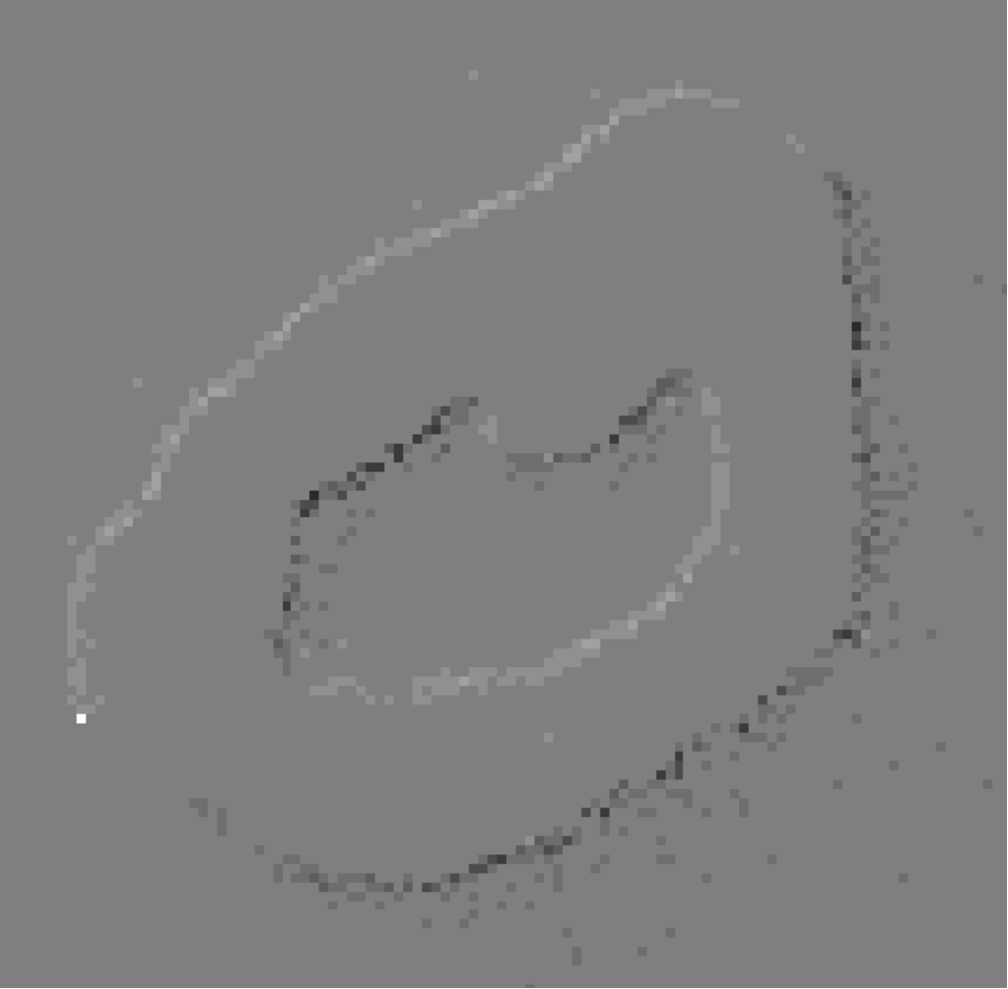
\includegraphics[width=0.22\textwidth]{dvs-128}
	}
	\subfloat[A snapshot of jAER playing Poissonian spike trains.]{
		\label{Fig:poisson}
		
\includegraphics[width=0.22\textwidth]{zero-28-2}
	}\\
	\subfloat[The raster plot of the Poissonian spike trains.]{
		\label{Fig:raster}
		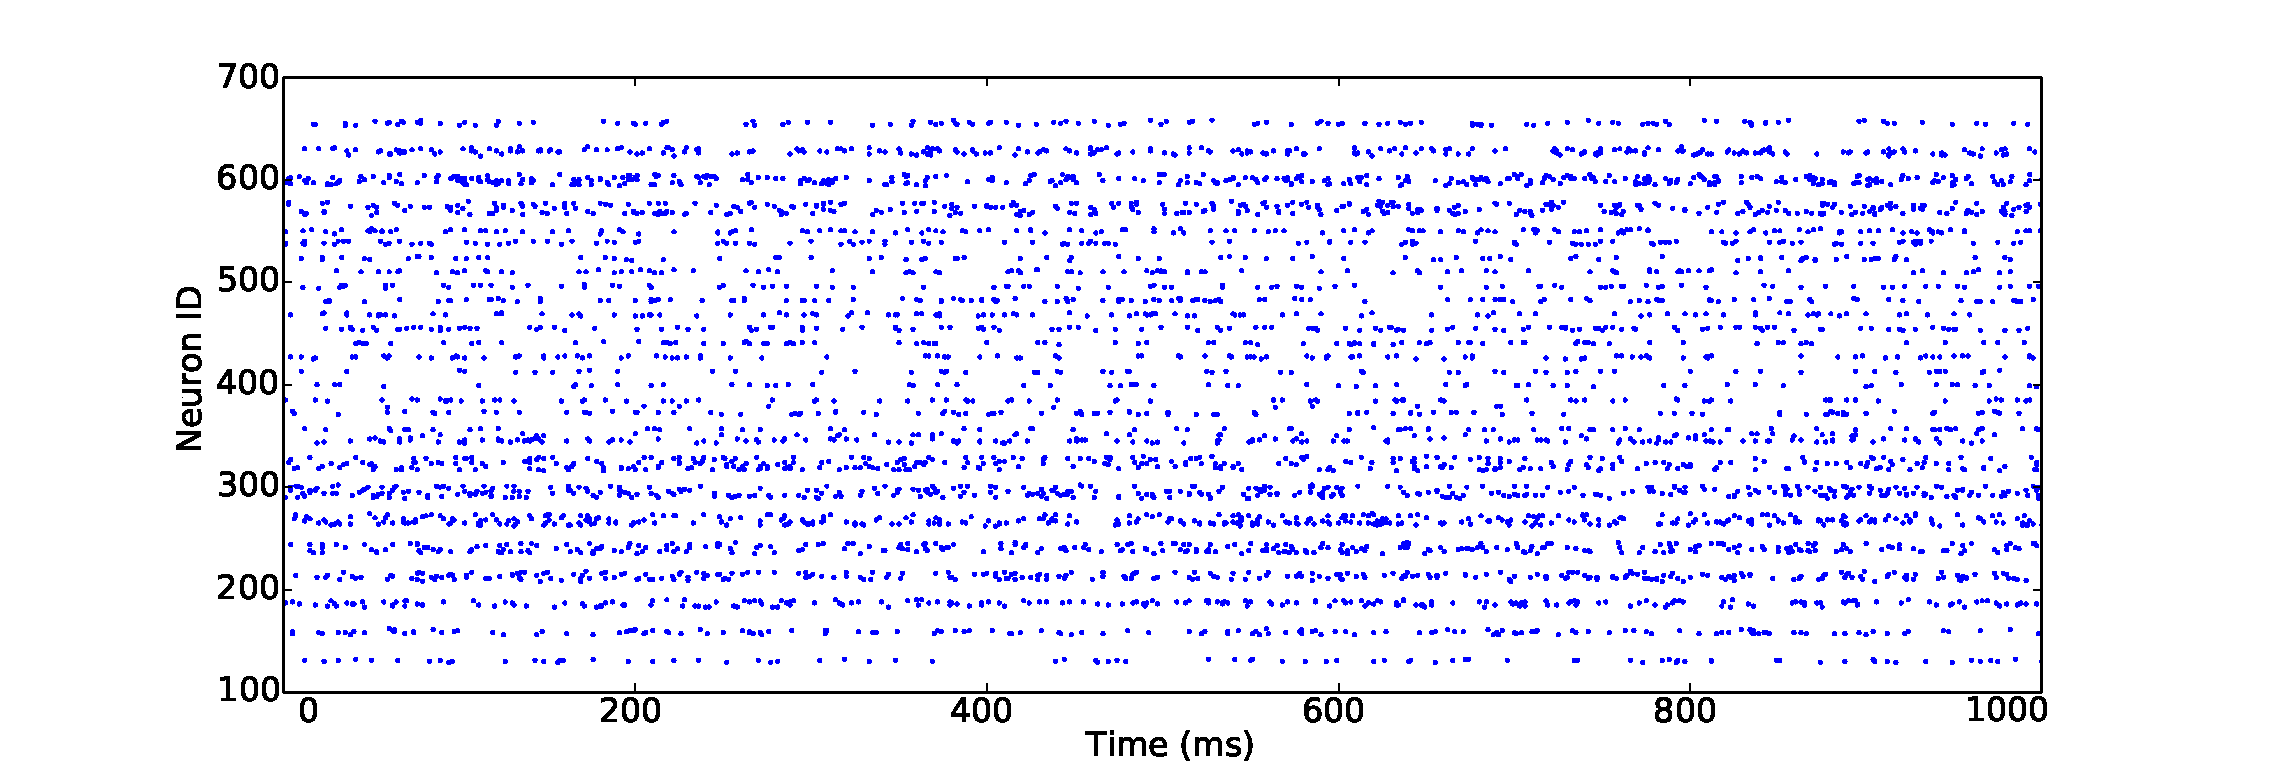
\includegraphics[width=0.48\textwidth]{zero}
	}
	
	\caption{
		Snapshots of jAER software playing spike presented videos.
		The same image of digit ``0'' is transformed to spikes by DVS recording and the Poissonian generation respectively.
		A raster plot of the Poissonian spike trains is also provided.}
	\label{fig:zero}
\end{figure}

\subsection{Data Description}	
\subsubsection{Poissonian}

In the cortex, the timing of spikes is highly irregular~\citep{squire1998findings}.
It can be interpreted that the inter-spike interval reflects a random process driven by the instantaneous firing rate.
If the generation of each spike is assumed to be independent of all the other spikes, the spike train is seen as a Poisson process.
The spiking rate can be estimated by averaging the pooled responses of the neurons.

As stated above, rate coding is exclusively used in presenting images with spikes.
The spiking rate of each neuron is in accordance with its corresponding pixel intensity.
Instead of providing exact spike arrays, we share the Python code for generating the spikes.
Every recognition system may require different spiking rates and various lengths of their durations.
The generated Poissonian spikes can be in the formats of both jAER and PyNN spike source array.
Thus, it is easy to visualise the digits and also to build spiking neural networks.
Because different simulators generate random Poissonian spike trains with various mechanisms, languages and codes, using the same dataset enables performance evaluation on different simulators without the interference created by non-unified input.
The same digit displayed in Fig.~\ref{Fig:jaer} is converted to Poissonian spike trains, see Fig.~\ref{Fig:poisson}.
The raster plot can be found in Fig.~\ref{Fig:raster}, indicating the intensities of the pixels.



\subsubsection{Rank-Order-Encoding}
A different way of encoding spikes is using a rank-order code; this means
keeping just the order in which those spikes were fired and disregarding the exact timing. Rank-ordered spike trains have been used in vision tasks under a biological plausibility constraint, making them a viable way of image encoding for neural applications~\citep{van2001rate,sen2009evaluating,masmoudi2010novel}.

Rank-ordered encoding can be performed using an algorithm known as the
{FoCal algorithm~\citep{sen2009evaluating}}.
It models the foveal pit region, the highest resolution area of the retina, with four ganglion cell layers that show a centre-surround behaviour~\citep{kolb2003retina}. In order to simulate these layers, four discrete 2D convolutions are performed. The centre-surround behaviour of the ganglion cells is modelled using Differences of Gaussians~(DoG). 
\begin{equation}
\label{eq-dog}
DoG_w(x,y) = \pm\frac{1}{2\pi\sigma_{w,c}^2}e^{\frac{-(x^2 + y^2)}{2\sigma_{w,c}^2}}
\mp\frac{1}{2\pi\sigma_{w,s}^2}e^{\frac{-(x^2 + y^2)}{2\sigma_{w,s}^2}}
\end{equation}
where $\sigma_{w,c}$ and $\sigma_{w,s}$ are the standard deviation for the 
centre and surround components of the DoG at layer $w$. The signs 
will be ($-$,$+$) if the ganglion cell has an OFF-centre behaviour and 
($+$,$-$) if it has an ON-centre one. Table~\ref{tab-kernel-specs} 
describes the parameters used to compute the convolution kernels at each 
scale $w$.

\begin{table}[htb]
	\caption{Simulation parameters for ganglion cells}
	\begin{center}
		
		
		\bgroup
		\def\arraystretch{1.4}
		
		\begin{tabular}{c c c c c c}
			\begin{minipage}{0.7cm}\centering Layer \end{minipage}& 
			\begin{minipage}{0.8cm}\centering Centre \\type \end{minipage}& 
			\begin{minipage}{0.7cm} \centering Matrix width \end{minipage}&  
			\begin{minipage}{1.3cm}\centering Centre std. dev. ($\sigma_c$)\vspace*{0.1cm}\end{minipage} & 
			\begin{minipage}{1.3cm}\centering Surround std. dev. ($\sigma_s$)\vspace*{0.1cm}\end{minipage} & 
			\begin{minipage}{1.3cm}\centering Sampling resolution (cols,rows)\vspace*{0.1cm}\end{minipage} \\
			\hline
			\begin{minipage}{0.7cm}\centering 1  \end{minipage} &
			\begin{minipage}{0.8cm}\centering OFF \vspace*{0.005cm} \end{minipage}& 
			\begin{minipage}{0.7cm}\centering$3$ \end{minipage}& 
			$0.8$ & $6.7 \times \sigma_c$ &  1, 1 \\
			\begin{minipage}{0.7cm}\centering 2 \end{minipage} & 
			\begin{minipage}{0.8cm}\centering ON \vspace*{0.005cm}\end{minipage} & 
			\begin{minipage}{0.7cm}\centering $11$ \end{minipage}& 
			$1.04$ & $6.7 \times \sigma_c$ & 1, 1 \\
			\begin{minipage}{0.7cm}\centering3 \end{minipage} &
			\begin{minipage}{0.8cm}\centering OFF \vspace*{0.005cm}\end{minipage} & 
			\begin{minipage}{0.7cm}\centering $61$ \end{minipage}& 
			$8$ & $4.8 \times \sigma_c$ & 5, 3 \\
			\begin{minipage}{0.7cm}\centering 4  \end{minipage} & 
			\begin{minipage}{0.8cm}\centering ON \vspace*{0.005cm}\end{minipage} & 
			\begin{minipage}{0.7cm}\centering $243$\end{minipage} &
			$10.4$ & $4.8 \times \sigma_c$ & 5, 3 
		\end{tabular}
		\egroup
	\end{center}
	\label{tab-kernel-specs}
\end{table}

Every pixel value in the convolved images (Fig. \ref{fig-convolution-results}) 
is inversely proportional to a spike emission time with respect to the presentation of the image (i.e. the higher the pixel value, the sooner the spike will be sent out.)

\begin{figure}[hbt]
	\centering
	\subfloat[Original image]{
		\label{sfig-rank-ordered-original}
		
\includegraphics[width=0.15\textwidth]{original_21-0}
	}
	\subfloat[Layer 1 (\textsc{off}-centre)]{
		\label{sfig-rank-ordered-midget-off}
		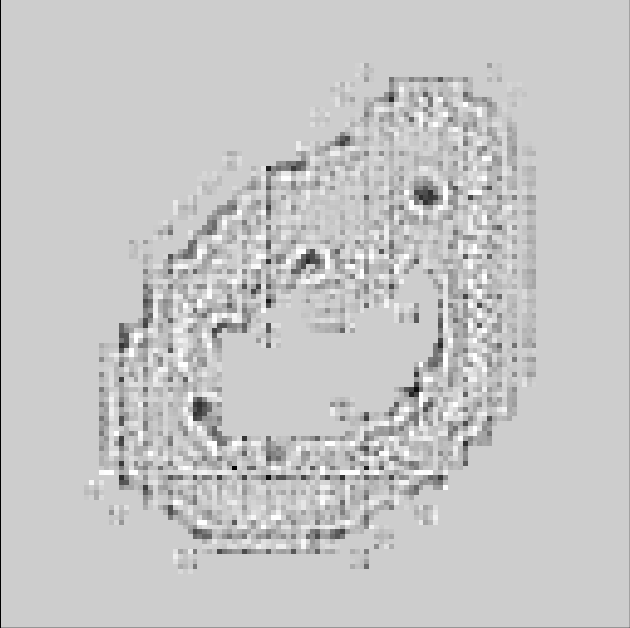
\includegraphics[width=0.15\textwidth]{filtered-21-0-layer-0}
	}
	\subfloat[Layer 2 (\textsc{on}-centre)]{
		\label{sfig-rank-ordered-midget-on}
		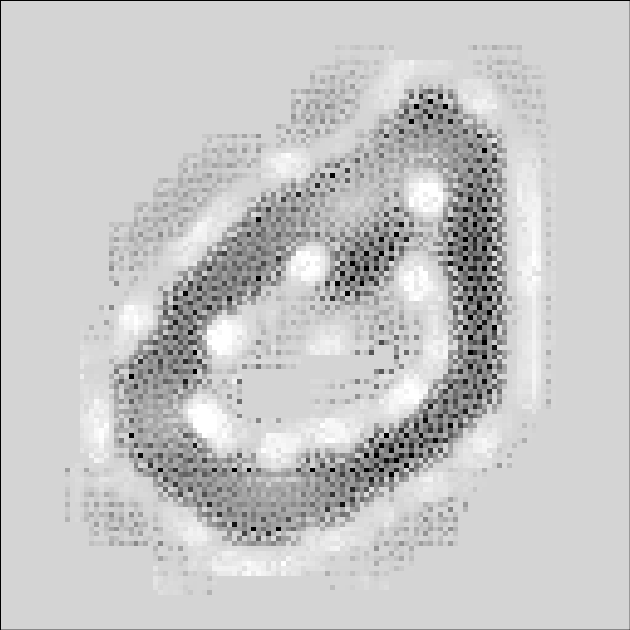
\includegraphics[width=0.15\textwidth]{filtered-21-0-layer-1}
	}\\
	\subfloat[Layer 3 (\textsc{off}-centre)]{
		\label{pic-lena-P-OFF}
		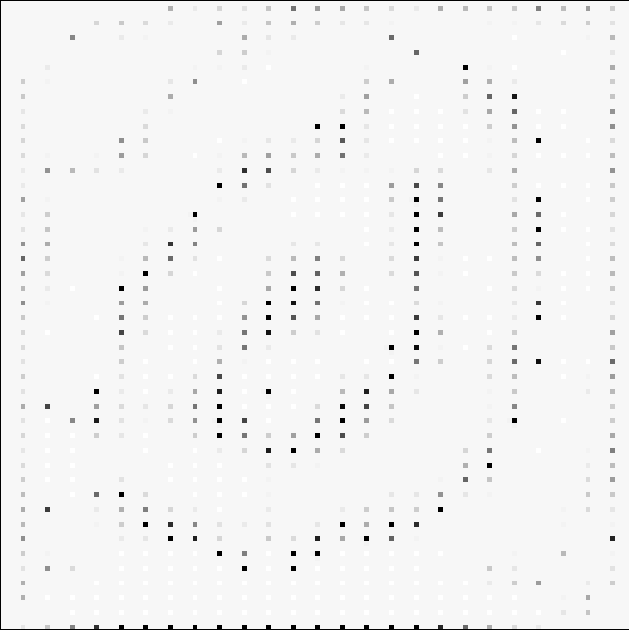
\includegraphics[width=0.15\textwidth]{filtered-21-0-layer-2}
	}
	\subfloat[Layer 4 (\textsc{on}-centre)]{
		\label{pic-lena-P-ON}
		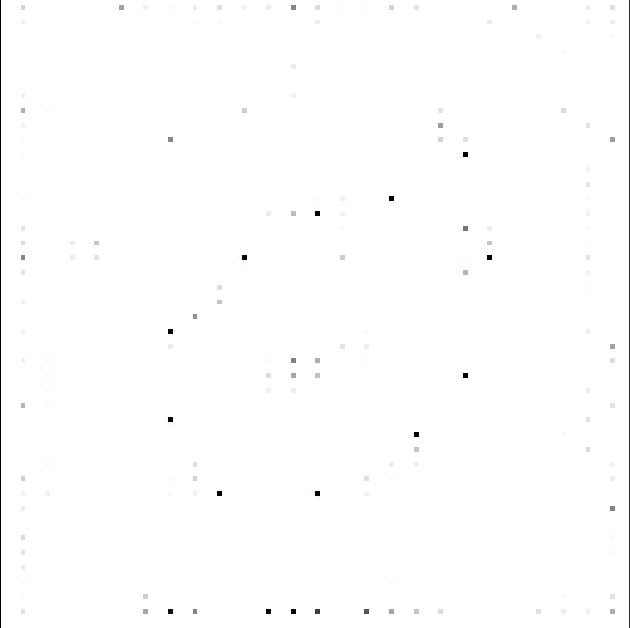
\includegraphics[width=0.15\textwidth]{filtered-21-0-layer-3}
	}
	\caption{Results of correcting the spikes from the simulated ganglion cell layers using the FoCal algorithms.}
	\label{fig-convolution-results}
\end{figure}
Since DoGs where used as a means to encode the image, and they are not an orthogonal basis, the algorithm also performs a redundancy correction step, it does so by 
adjusting the convolved image's pixel value according to the correlation 
between convolution kernels (Alg.~\ref{code-focal-corr}).
\begin{algorithm}[h]
	\caption{FoCal, redundancy correction}
	\label{code-focal-corr}
	\begin{algorithmic}
		\Procedure{Correction}{coeffs $C$, correlations $Q$}
		\State $N \leftarrow \emptyset$ \Comment{Corrected coefficients}
		\Repeat
		\State $m \leftarrow max(C)$\Comment{Obtain maximum from $C$}
		\State $M \leftarrow M \cup m$\Comment{Add maximum to $M$}
		\State $C \leftarrow C \setminus m$\Comment{Remove maximum from $C$}
		\ForAll{$ c \in C$} \Comment{Adjust all remaining $c$}
		\If{$Q(m, c) \neq 0$} \Comment{Adjust only near}
		\State $c \leftarrow c - m \times Q(m, c)$
		\EndIf
		\EndFor
		\Until{$C = \emptyset$}
		\State \textbf{return} $M$
		\EndProcedure
	\end{algorithmic}
\end{algorithm}


After the correction step, the most important information can be recovered using only the first 30\% of the spikes~\citep{sen2009evaluating}. These significant spikes are shown in Fig.~\ref{fig-raster-plot-30pc}, assuming that each spike will be generated 1~ms apart. Neurons in Layer 1 emit spikes faster and in larger quantities than any other layer, making it the most important one. Layers 2 and 3 have few spikes, this is due to the large convolution kernels used to simulate the ganglion cells. One of the main advantages of ROC is that neurons will only spike once, this can be seen particularly well in these two layers. Layers 0 and 1 encode fine details, while layers 2 and 3 result in blob like features.
\begin{figure}[hbt]
	\centering
	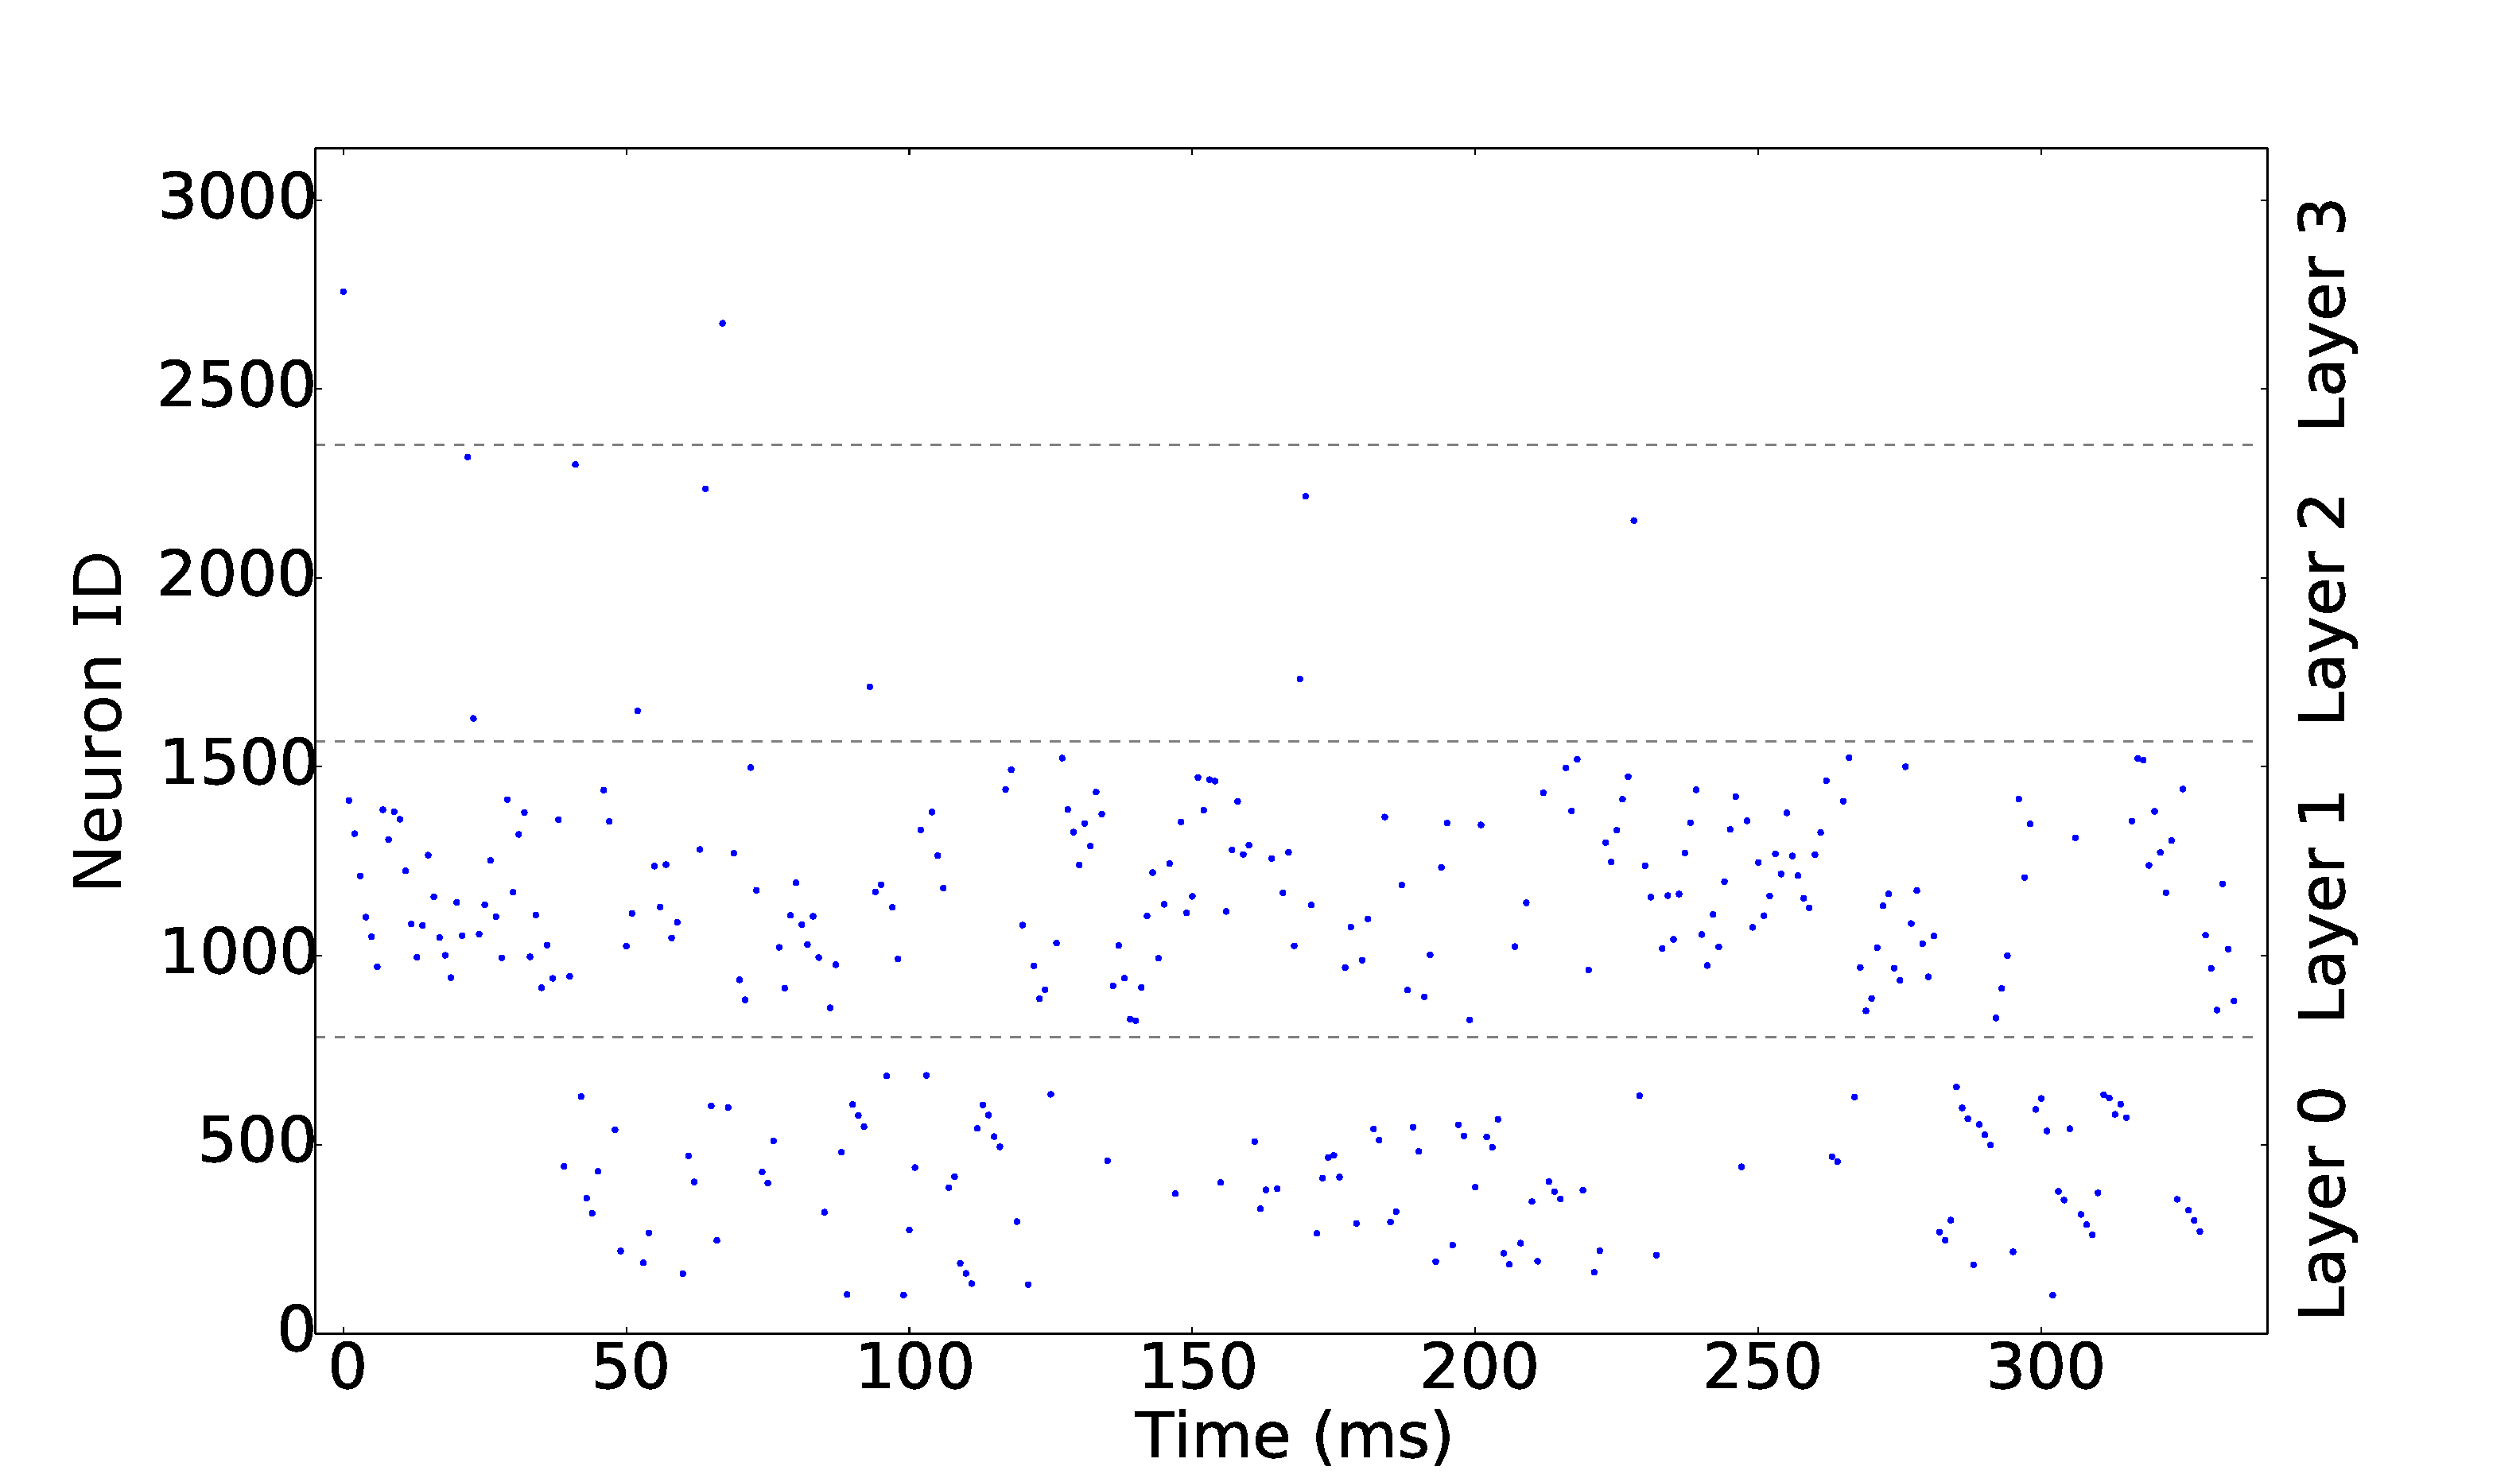
\includegraphics[width=0.475\textwidth]{raster-plot-21-0-30pc}
	\caption{First 30\% of the rank-order encoded spikes produced with FoCal.}
	\label{fig-raster-plot-30pc}
\end{figure}

Figure \ref{fig-reconstruction-results} shows the reconstruction results for the two stages of the algorithm. On Fig. \ref{pic-lena-reconstructed-raw} the reconstruction was applied after the convolution but without the FoCal correction, a blurry image is the result of redundancy in the spike representation. A better reconstruction can be obtained after Algorithm \ref{code-focal-corr} has been applied, the result is shown in Figure \ref{pic-lena-reconstructed-focal}.


\begin{figure}[hbt]
	\centering
	\subfloat[Original image]{
		\label{sfig-rank-ordered-original-1}
		
\includegraphics[width=0.15\textwidth]{original_21-0}
	}
	\subfloat[No correction]{
		\label{pic-lena-reconstructed-raw}
		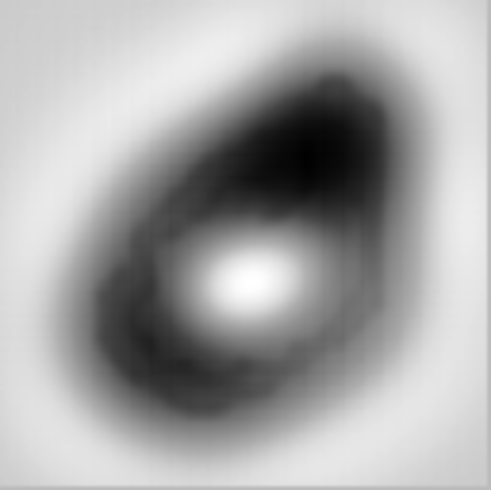
\includegraphics[width=0.15\textwidth]{reconstructed_21-0_raw}
	}
	\subfloat[FoCal]{
		\label{pic-lena-reconstructed-focal}
		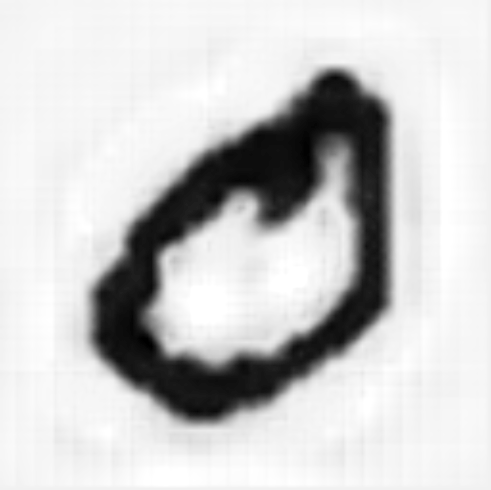
\includegraphics[width=0.15\textwidth]{reconstructed_21-0_100pc}
	}
	\caption{Reconstruction result comparison.}
	\label{fig-reconstruction-results}
\end{figure}

The source Python scripts to transform images to ROC spike trains, and to convert the results into AER and PyNN's spike source array can be found in the dataset's website.
\subsubsection{DVS Sensor Output with Flashing Input}
\label{subsec_flash}
The purpose of including the subset of DVS recorded flashing digits is to promote the application of Rank-Order-Coding to DVS output, and accelerate the fast on-set recognition by using just the beginning part of spike trains within less than 30~ms.

Each digit and a blank image was shown alternately and each display lasted one second.
The digits were displayed on an LCD monitor in front of the DVS retina~\citep{serrano2013128} and were placed in the centre of the visual field of the camera.
Since there are two polarities of the spikes: 'ON' indicates the increase of the intensity while 'OFF' reflects the opposite, there are 'ON' and 'OFF' flashing recordings respectively per digit.
In Fig.~\ref{fig:flash}, the burstiness of the spikes is illustrated where most of the spikes occur in a 30~ms slot. 
In total, the subset of the database contains 2$\times$$60,000$ recordings for training and 2$\times$$10,000$ for testing.

\begin{figure}[b!]
	\centering
	\subfloat[Spikes recorded in the order of neuron ID during 1s of time.]{
		\label{fig:flash_all}
		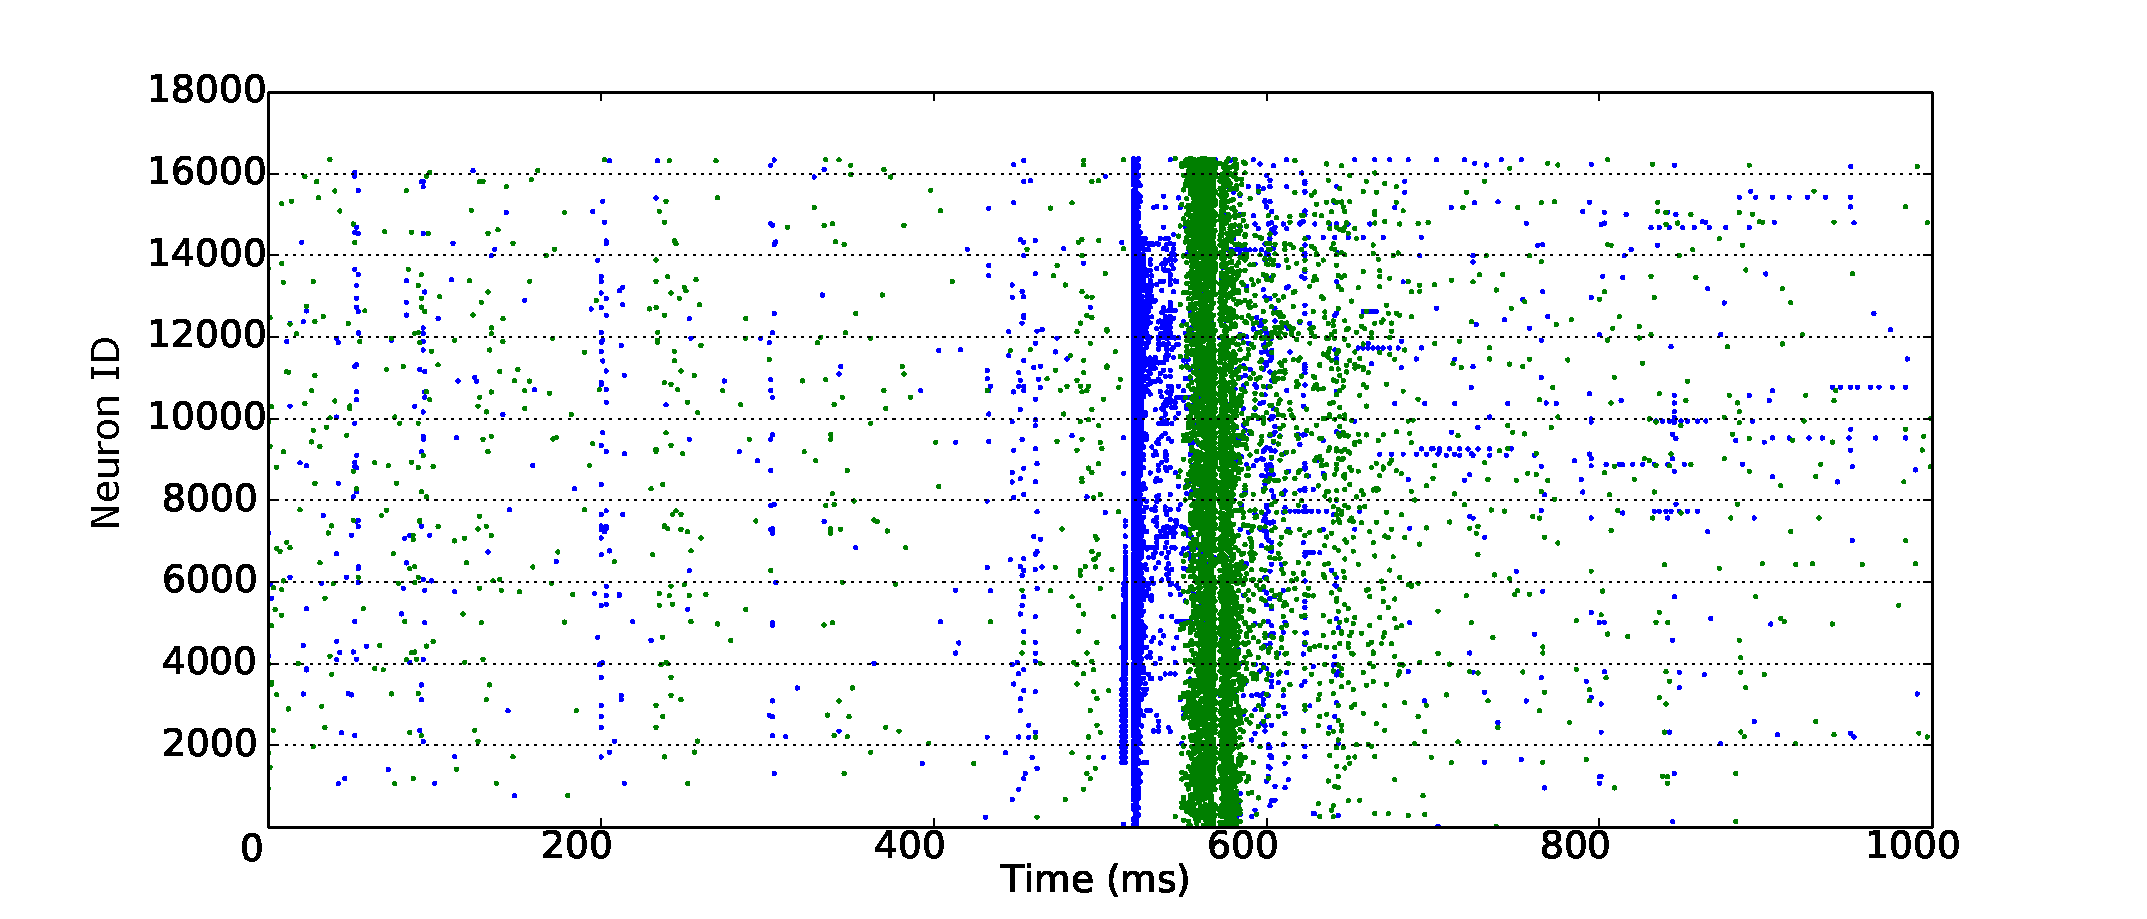
\includegraphics[width=0.48\textwidth]{flash_full}
	}
	\\
	\subfloat[Spikes plotted in the sequence of appearing time during 1s of time. Bursty spikes apeer in slots less than 30~ms. ]{
		\label{fig:flash_a}
		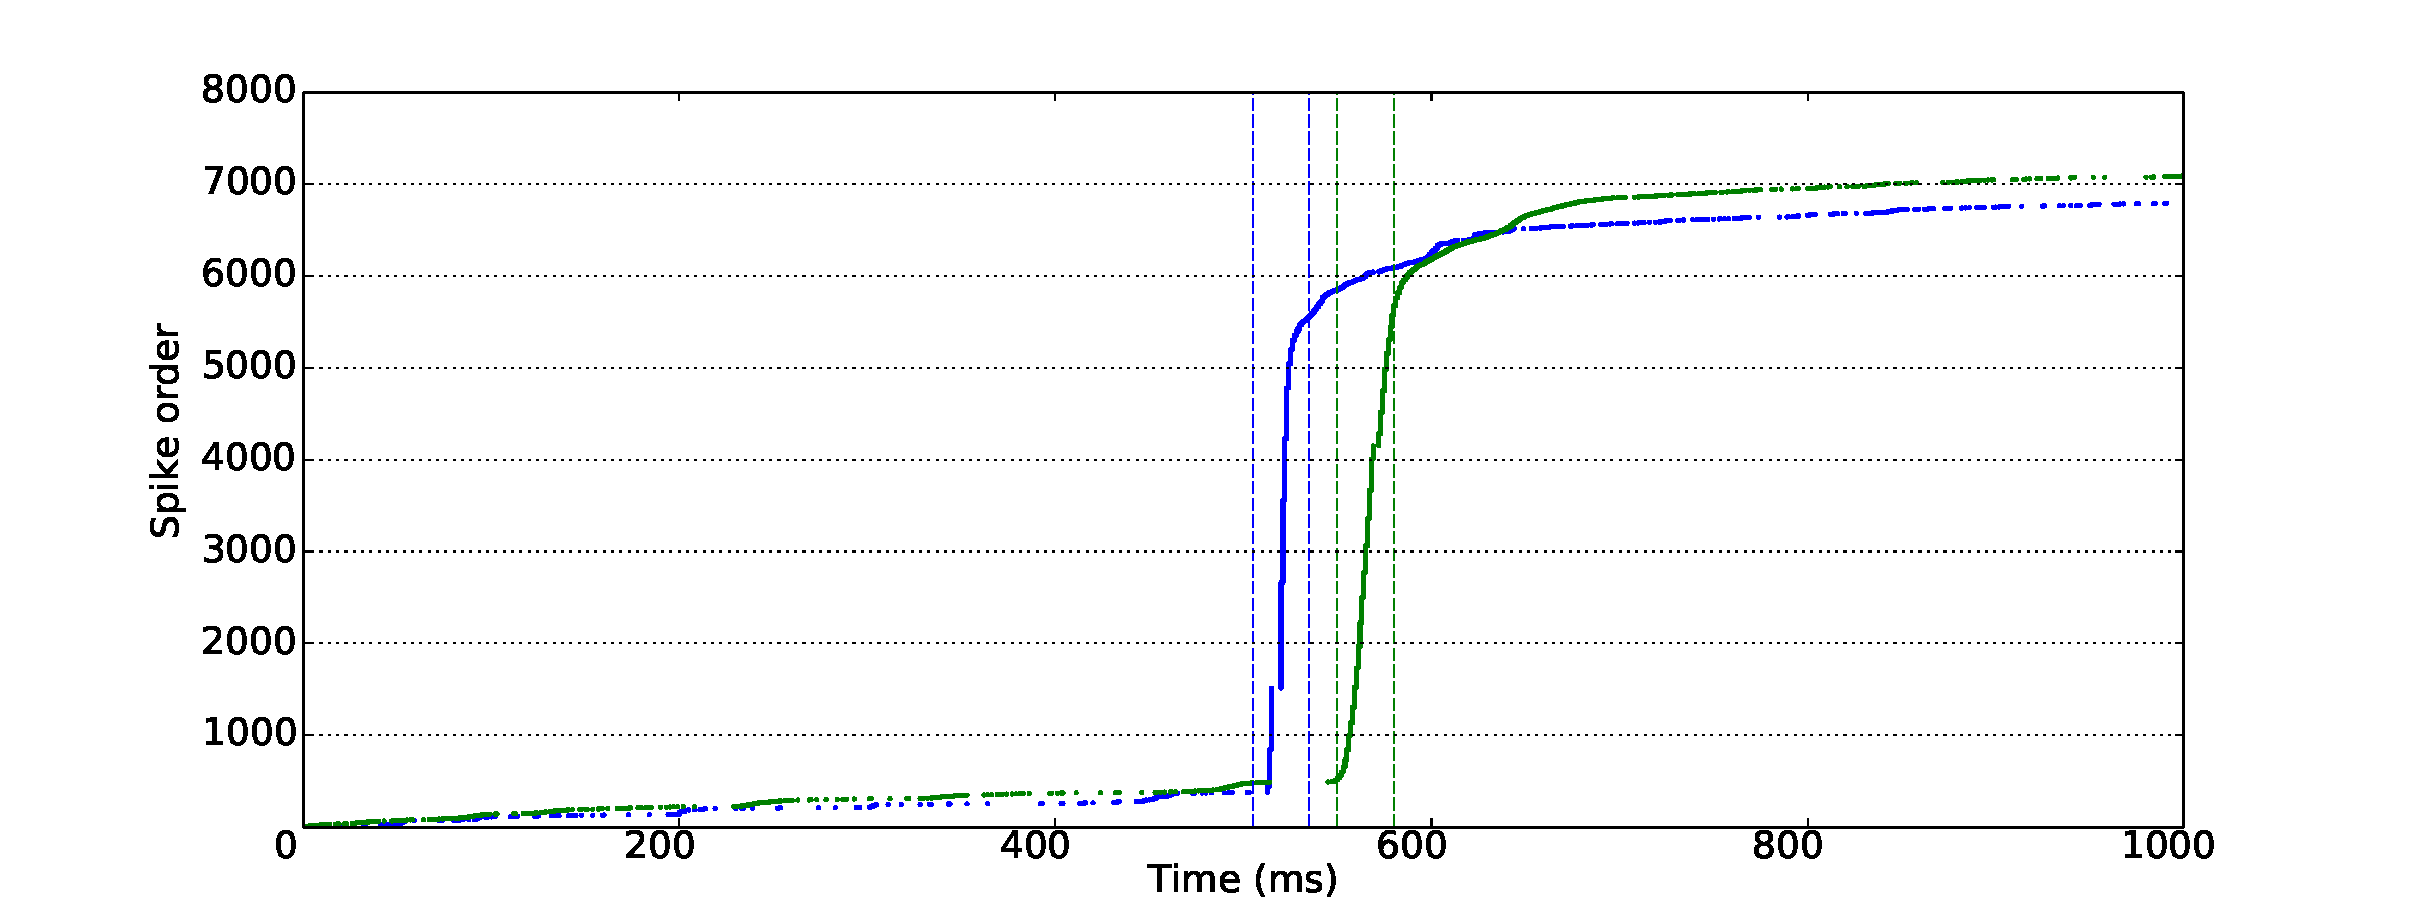
\includegraphics[width=0.48\textwidth]{flash_full_order}
	}
	
	\caption{The bursty of spikes is illustrated where most of the spikes occur in a 30~ms slot. Blue for 'ON' events and green for 'OFF'.}
	\label{fig:flash}
\end{figure}

\subsubsection{DVS Sensor Output with Moving Input}
In order to address the problems of position- and scale- invariance, a subset of DVS recorded moving digits is presented.

MNIST digits were scaled to three different sizes, by using smooth interpolation algorithms to increase their size from the original 28x28 pixel size, and displayed on the monitor with slow motion. 
The same DVS~\citep{serrano2013128} used in Section~\ref{subsec_flash} captured the movements of the digits and generated spike trains for each pixel of its 128$\times$128 resolution.
A total of 30,000 recordings were made: 10 digits, at 3 different scales, 1000 different handwritten samples for each.

\section{Performance Evaluation}
\label{sec:eval}
A complementary evaluation methodology is essential to provide common metrics and assess both the model-level and hardware-level performance.

\begin{table*}[hbt!]
	\caption{Hardware independent comparison}
	\begin{center}
		\bgroup
		\def\arraystretch{1.5}
		\begin{tabular}{ l c c c c }
			$ $ &
			\begin{mycell}{1.9cm}Preprocessing\end{mycell} & 
			\begin{mycell}{3.5cm} Network\end{mycell} & 
			\begin{mycell}{3.5cm} Training \end{mycell} & 
			\begin{mycell}{3.5cm} Recognition \end{mycell} \\
			\hline
			
			%
			\begin{mycell}{2.5cm}~\cite{brader2007learning} \end{mycell} & 
			\begin{mycell}{1.9cm} None \end{mycell} & % preprocessing
			\begin{mycell}{3.5cm} Two layer, LIF neurons\end{mycell}&  % network
			\begin{mycell}{3.5cm} Semi-supervised, STDP, calcium LTP/LTD\end{mycell}&  % training
			\begin{mycell}{3.5cm} 96.5\% \end{mycell} \\% recognition
			
			%
			\begin{mycell}{2.5cm}~\cite{beyeler2013categorization} \end{mycell} & 
			\begin{mycell}{1.9cm} None \end{mycell} & % preprocessing
			\begin{mycell}{3.5cm} V1 (edge), \\V4 (orientation),\\ and competitive decision, Izhikevich neurons\end{mycell}&  % network
			\begin{mycell}{3.5cm} Semi-supervised, STDP, \\ calcium LTP/LTD \end{mycell} &  % training
			\begin{mycell}{3.5cm} 91.6\% \\ 300~ms per test \end{mycell} \\% recognition
			
			%
			\begin{mycell}{2.5cm}~\cite{neftci2013event} \end{mycell} & 
			\begin{mycell}{1.9cm} Thresholding\end{mycell} & % preprocessing
			\begin{mycell}{3.5cm} Two layer RBM, \\ LIF neurons \end{mycell}&  % network
			\begin{mycell}{3.5cm} Event-driven contrastive divergence, supervised \end{mycell}&  % training
			\begin{mycell}{3.5cm} 91.9\% \\ 1~s per test\end{mycell} \\% recognition
			
			%
			\begin{mycell}{2.5cm}~\cite{diehl2015unsupervised} \end{mycell} & 
			\centering None &
			\begin{mycell}{3.5cm} Two layers, LIF neurons, inhibitory feedback  \end{mycell}& 
			\begin{mycell}{3.5cm} Unsupervised, exp. STDP, %adaptive membrane potential, 
				$3,000,000$~s of training\\ $200,000$~s per iteration\end{mycell} & 
			\begin{mycell}{3.5cm} 95\% \end{mycell}\\
			
			%
			\begin{mycell}{2.5cm}~\cite{Diehl2015fast}\end{mycell}  & 
			\begin{mycell}{1.9cm} None \end{mycell} & % preprocessing
			\begin{mycell}{3.5cm} ConvNet or \\Fully Connected (FC) net,\\ LIF neurons \end{mycell}& % network
			\begin{mycell}{3.5cm} Off-line trained with ReLU, weight normalization \end{mycell}&   % training
			\begin{mycell}{3.5cm} 99.1\% (ConvNet), \\ 98.6\% (FC net);\\0.5~s per test\end{mycell}\\ % recognition    
			%
			\begin{mycell}{2.5cm}~\cite{zhao2014feedforward}\end{mycell}  & 
			\begin{mycell}{1.9cm} Thresholding\\ or DVS \end{mycell}& % preprocessing 
			\begin{mycell}{3.5cm} Simple (Gabor), \\Complex (MAX) \\and Tempotron  \end{mycell}& % network
			\begin{mycell}{3.5cm} Tempotron, supervised \end{mycell}& % training
			\begin{mycell}{3.5cm} Thresholding \\ 91.3\%, 11~s per test \\ DVS \\ 88.1\%, 2~s per test\end{mycell}\\ % recognition
			
			%
			\begin{mycell}{2.5cm} % %\cite{Stromatias2015scalable} \\ 
				This paper \end{mycell} & 
			\begin{mycell}{1.9cm} None \end{mycell} & % preprocessing
			\begin{mycell}{3.5cm} Four layer RBM, \\ LIF neurons \end{mycell}&  % network
			\begin{mycell}{3.5cm} Off-line trained, unsupervised \end{mycell}&  % training
			\begin{mycell}{3.5cm} 94.94\%\\16 ms latency \end{mycell} \\% recognition
			%
			\begin{mycell}{2.5cm} This paper \end{mycell}  & 
			\begin{mycell}{1.9cm} None \end{mycell}& % preprocessing 
			\begin{mycell}{3.5cm} FC decision layer, \\ LIF neurons \end{mycell}& % network
			\begin{mycell}{3.5cm} K-means clusters,\\Supervised STDP\\$18,000$~s of training \end{mycell}& % training
			\begin{mycell}{3.5cm} 92.98\%\\1~s per test\\10.70~ms latency\end{mycell}\\ % recognition
		\end{tabular}
		\egroup
	\end{center}
	\label{tb:software_comparison}
\end{table*}

\subsection{Hardware-Independent}
\label{subsec:model}


First of all it is desirable for researchers to specify whether they add any preprocessing either to images or spikes.
Filtering the raw input may ease the classification/recognition task while adding noise may require stronger robustness of the model.
Secondly, as with the evaluation on conventional artificial neural networks, a description of the network characteristics is most welcome since it is the basis for the overall performance.
Furthermore, sharing the designs may inspire fellow scientists to bring new points of view to the problem and generate a positive feedback loop where everybody wins.
The network description should include the topology, and the neural and synaptic models.
The network topology defines the number of neurons used for each layer, and the connections between layers and neurons.
Some researchers make use of extra non-neural classifiers, sometimes to aid the design, others to enhance the output of the network.
Any particulars on this subject are greatly appreciated.
It is essential to state the type of neural and synaptic model (e.g. current-based LIF neuron) exploited in the network and the parameters configuring them, because neural activities differ greatly between various configurations.
Thirdly, the learning procedure determines the recognition capability of a network model.
A clear distinction has always been made between supervised, semi-supervised and unsupervised learning.
A detailed description of new proposed spike-based learning rules will be a great contribution to the field due to the lack of spatio-temporal learning algorithms.
Most publications reflect the use of adaptations to existing learning rules, details on the modifications are highly desired.
In conventional computer vision, iterations of training images presented to the network play an important role.
Similarly, the biological time of training decides the amount of information provided.

Finally in the testing phase where performance evaluation takes place, specific measurements of SNN models are essential in addition to recognition accuracy.
It should include details of the way samples were presented: event rates, and biological time per testing sample.
The combination of these two factors determines how much information is presented to the network.
An important performance metric is the response time (latency) of an SNN model.
A faster model is more suitable for real-time recognition systems such as neuromorphic robotics.
A commonly reported characteristic is the accuracy of the network, perhaps adding remarks on how these scores are obtained could help to unify criteria and ease comparison.
Work on SNN-based classifications of MNIST are listed in Table~\ref{tb:software_comparison} and evaluated on the proposed metrics.

\subsection{Hardware-Specific}
\label{subsec:hw}

  \begin{table*}[thb!]
  	\caption{Hardware dependent comparison}
  	\begin{center}
      \begin{minipage}{\textwidth}
        
        \begin{savenotes}
  		\bgroup
  		\def\arraystretch{1.4}
  		\begin{tabular}{l c c c c c c}
  			$ $ & 
  			\begin{mycell}{2.0cm} System \end{mycell} & 
  			%       \begin{minipage}{1.3cm}\centering Simulation type \end{minipage} & 
  			
  			\begin{mycell}{2.0cm} Neuron Model \end{mycell} & 
  			\begin{mycell}{2.0cm}Synaptic\\Plasticity\end{mycell} &
  			%       \begin{minipage}{1cm}\centering Axonal delays \end{minipage} & 
  			%       \begin{minipage}{1cm}\centering Synaptic model \end{minipage} & 
  			\begin{mycell}{2.0cm} Precision \end{mycell} &  
  			%       \begin{minipage}{1.2cm}\centering Synaptic precision \end{minipage} & 
  			%       \begin{minipage}{1.2cm}\centering Energy per SE \end{minipage} & 
  			%       \begin{minipage}{1.4cm}\centering Synaptic ops per Watt \end{minipage} & 
  			\begin{mycell}{2.0cm} Simulation\\Time \end{mycell} & 
  			\begin{mycell}{2.0cm} Energy/Power \\Usage \end{mycell} 
  			%       \begin{minipage}{1.7cm}\centering Programming front-end \end{minipage}  
  			\\
  			\hline
  			% contents!
  			
  			\begin{mycell}{1.8cm} SpiNNaker \citep{stromatias2013power} \end{mycell} &
  			\begin{mycell}{2.0cm} Digital, \\Scalable \end{mycell} & 
  			\begin{mycell}{2.1cm}Programmable\\Neuron/Synapse,\\Axonal delay \end{mycell}& 
  			\begin{mycell}{2.1cm}Programmable\\learning rule\end{mycell}& 
  			\begin{mycell}{2.0cm}11- to 14-bit synapses\end{mycell} & 
  			\begin{mycell}{2.0cm} Real-time \\ Flexible time resolution \end{mycell}  &
  			\begin{mycell}{2.5cm} 8~nJ/SE \\54.27 MSops/W \end{mycell} \\
  			%
  			\begin{mycell}{1.8cm} TrueNorth \citep{merolla2014million}\end{mycell} & \begin{mycell}{2.0cm}Digital, \\Scalable \end{mycell}& 
  			\begin{mycell}{2.0cm}Fixed models,\\Config params,\\Axonal delay\end{mycell}& 
  			\begin{mycell}{2.0cm}No plasticity\end{mycell}& 
  			\begin{mycell}{2.2cm}122 bits \\params \& states,
  				%       	 per neuron
  				\\ 4-bit synapse 
  				%\\(4 signed int + on/off state)
          \footnote[1]{We consider them 4-bit synapses because it is only possible to choose between 4 different signed integers and whether the synapse is active or not.}
  			\end{mycell}& 
  			\begin{mycell}{2.0cm}Real-time\end{mycell}& 
  			\begin{mycell}{2.0cm}46 GSops/W\end{mycell} \\
  			
  			%
  			\begin{mycell}{1.8cm} Neurogrid \citep{benjamin2014neurogrid}\end{mycell} &
  			\begin{mycell}{2.0cm}Mixed-mode,\\Scalable\end{mycell} & 
  			\begin{mycell}{2.0cm}Fixed models,\\Config params\end{mycell} & 
  			\begin{mycell}{2.0cm}Fixed rule\end{mycell} & 
  			\begin{mycell}{2.0cm}13-bit shared \\ synapses\end{mycell} &
  			\begin{mycell}{2.0cm}Real-time\end{mycell} &
  			\begin{mycell}{2.0cm}941 pJ/SE\end{mycell} \\
  			%
  			\begin{mycell}{1.8cm} HI-CANN \citep{schemmel2010wafer}  \end{mycell} & \begin{mycell}{2.0cm}Mixed-mode,\\Scalable\end{mycell} &
  			\begin{mycell}{2.0cm}Fixed models,\\Config params\end{mycell}& 
  			\begin{mycell}{2.0cm}Fixed rule\end{mycell}& 
  			\begin{mycell}{2.0cm}4-bit synapses\end{mycell}& 
  			\begin{mycell}{2.0cm}Faster than\\ real-time
                             \footnote[2]{A speed-up of up to $10^5$ times real time has been reported.}
        \end{mycell}&
  			\begin{mycell}{2.0cm}198 pJ/SE \\ 13.5 MSops/W \\(network only) \end{mycell}\\
  			%
  			\begin{mycell}{1.8cm} HiAER-IFAT \citep{yu201265k}\end{mycell} & 
  			\begin{mycell}{2.0cm}Mixed-mode,\\Scalable\end{mycell} &
  			\begin{mycell}{2.0cm}Fixed models,\\Config params\end{mycell}& 
  			\begin{mycell}{2.0cm}No plasticity\end{mycell} &  
  			\begin{mycell}{2.0cm}Analogue neuron/synapse\end{mycell} & 
  			Real-time&
  			\begin{mycell}{2.0cm}22-pJ/SE\\\citep{park201465k}\\20GSops/W\end{mycell}
  			
  			%dummy update text
  		\end{tabular}
  		\egroup

\end{savenotes}
\end{minipage}
  	\end{center}
  	\label{tb:hardware_comparison}
  \end{table*}


Depending on how neurons, synapses and spike transmission are implemented neuromorphic systems can be categorised as either analogue, digital, or mixed-mode analogue/digital VLSI circuits. Some analogue implementations exploit sub-threshold transistor dynamics to emulate neurons and synapses directly on hardware~\citep{indiveri2011neuromorphic} and are more energy-efficient while requiring less area than their digital counterparts~\citep{joubert2012hardware}. However, the behaviour of analogue circuits is largely determined during the fabrication process due to transistor mismatch~\citep{indiveri2011neuromorphic,pedram2006thermal,linares2003compact}, while their wiring densities render them impractical for large-scale systems. The majority of mixed-mode analogue/digital neuromorphic platforms, such as the High Input Count Analog Neural Network (HI-CANN)~\citep{schemmel2010wafer}, Neurogrid~\citep{benjamin2014neurogrid}, HiAER-IFAT~\citep{yu201265k}, use analogue circuits to emulate neurons and digital packet-based technology to communicate spikes as AER events. This enables reconfigurable connectivity patterns, while the time of spikes is expressed implicitly since typically a spike reaches its destination in less than a millisecond, thus fulfilling the real-time requirement. Digital neuromorphic platforms such as TrueNorth~\citep{merolla2014million} use digital circuits with finite precision to simulate neurons in an event driven manner to minimise the active power dissipation. Neuromorphic systems suffer from model flexibility, since neurons and synapses are fabricated directly on hardware with only a small subset of parameters exposed to the researcher. 
SpiNNaker is a biologically inspired, massively-parallel, scalable computing architecture designed by the Advanced Processor Technologies (APT) group at the University of Manchester. SpiNNaker has been optimised to simulate very large-scale spiking neural networks in real-time~\citep{furber2014spinnaker}. SpiNNaker aims to combine the advantages of conventional computers and neuromorphic hardware by utilising low-power programmable cores and scalable event-driven communications hardware.

A direct comparison between neuromorphic platforms is a non-trivial task due to the different hardware implementation technologies as mentioned above.
%Qian Liu modified
The metric proposed in Table~\ref{tb:hardware_comparison} attempts to expose the advantages and disadvantages of different neuromorphic hardware thus to find out the network properties each platform is suited to.
The scalability of a hardware platform determines the network size limit of a neural application running on it.
Considering the various neural, synaptic models, plasticity learning rules and lengths of axonal delays, a programmable platform is flexible for diverse SNNs while a hard-wired system supporting only specific models wins for its simpler design and implementation.
The classification accuracy of a SNN running on a hardware system can be different from the software simulation, since hardware implementation limits on the precision used for the membrane potential of neurons (for the digital platforms) and the synaptic weights.
Thus comparison metrics is supposed to include precision as a major assessment of the system performance.
Simulation time is another important measure of running large-scale networks on hardware.
Real-time implementation is an essential requirement for robotic systems because of the real-time input from the neuromorphic sensors.
Running faster than real time is attractive for large/long simulations.
However, due to the limitation of hardware resources simulation time may accelerate or slow down according to the network topology and spike dynamics.
Also finer time resolution plays an important role in precision sensitive neural models or in sub-millisecond tasks~\citep{lagorce2015breaking}.
%Qian Liu done
Comparing the performance of each platform in terms of energy requirements is an interesting comparison metric especially if targeted for mobile applications and robotics. Some researchers have suggested the use of energy per synaptic event (J/SE)~\citep{sharp2012power,stromatias2013power} as an energy metric because the large fan in and out of a neuron tend to dominate the total energy dissipation during a simulation. Merolla et al. proposed the number of synaptic operations per Watt (Sops/W)~\citep{merolla2014million}.
These two measurements are the same presentations of energy use of synaptic events, since J/SE$\times$Sops/W = 1 s. 

%Qian Liu modified
For a particular SNN application or benchmark, the scalability and programmability will determine whether the network is able to run on a platform.
The system performance will be assessed on the accuracy, simulation time and energy use running the network. 
Table~\ref{tb:hardware_comparison} aims to summarise the aforementioned hardware comparison metrics.

\section{Case Studies}
\label{sec:test}
In this section, we present two recognition SNN models working on the Poissonian subset of the NE15-MNIST dataset.
Their network components, training and testing methods are described according to the evaluation methodology stated above.
The specific spike-based evaluations on input event rates and/or responding latency are also provided. 
Meanwhile, as tentative benchmarks the models are implemented on SpiNNaker to assess the performance against software simulators.
Presenting proper benchmarks for vision recognition systems is still under investigation, the case studies only make first attempt.

\subsection{Case Study I}
The first case study is a simple two-layered network where the input neurons receive Poissonian presented spike trains from the dataset and form a fully connected (FC) network with the decision neurons.
The model utilises LIF neurons, and the parameters are all with biological means, see the listed values in Table~\ref{tbl:pynnSetting}.
The LIF neuron model follows the membrane potential
dynamics:
\begin{equation}
\tau_m \frac{\D V}{\D t}=V_{rest} - V + R_{m} I_{syn}(t) ~~~,
\label{eq:LIF}
\end{equation}
where $\tau_m$ is the membrane time constant, $ V_{rest} $ is the resting potential, $ R_{m} $ is the membrane resistance and $ I_{syn} $ is the synaptic input current.
In PyNN, $ R_{m} $ is presented by $ R_{m}=\tau_m/C_{m} $, where $C_{m} $ is the membrane capacitance.
A spike is generated when the membrane potential goes beyond the threshold, $ V_{thresh} $ and the membrane potential resets to $V_{reset}$.
In addition, a neuron cannot fire within the refractory period, $ \tau_{refrac} $, after generating a spike.

The connections between the input neurons and the decision neurons are plastic, so the connection weights can be modulated during training with a standard STDP learning rule.
The model is described with PyNN and the code is published in
%\footnote {https://github.com/qian-liu/benchmarking/tree/master/code/case\_study\_I}
the same Github repository with the dataset.
As a potential benchmark, this system is composed with simple neural models, trained with standard learning rules and written in a unified SNN description language. These characteristics allow the same network to be tested on various simulators, both software- and hardware-based.

Both the training and testing exploit the Poissonian subset of the NE15-MNIST dataset.
This makes performance evaluation on different simulators possible with the unified spike source array provided by the dataset. 
In terms of this case study, the performance of the model was evaluated with both software simulation [on NEST~\citep{gewaltig2007nest}] and hardware implementation (on SpiNNaker).

In order to fully assess the performance, different settings have been configured on the network, such as network size, input rate and testing images duration.
For simplicity of describing the system, one standard configuration is set as the example in the following sections.
\begin{table}[hbbp]
	\centering
	\caption{\label{tbl:pynnSetting}Parameter setting for the current-based LIF neurons using PyNN.}
	\bgroup
	\def\arraystretch{1.1}
	\begin{tabular}{c|c|c}
		%\hline
		Parameters & Values & Units \\
		\hline
		cm & 0.25 & nF	\\
		%\hline
		tau\_m & 20.0 & ms\\
		%\hline
		tau\_refrac & 2.0 & ms\\
		%\hline
		%  tau\_syn\_E & 1.0 & ms\\
		%  %\hline
		%  tau\_syn\_I & 1.0 & ms\\
		%  %\hline
		v\_reset & -70.0 & mV\\
		%\hline
		v\_rest & -65.0 & mV\\
		%\hline
		v\_thresh & -50.0 & mV\\
		%\hline
	\end{tabular}
	\egroup
\end{table}

\subsubsection{Training}
There are two layers in the model: 28$\times$28 input neurons fully connect to 100 decision neurons.
Each decision neuron responds to a certain template of a digit.
In the standard configuration, there are 10 decision neurons answering to the same digit with slightly different templates.
Those templates are embedded in the connection weights between the two layers.
Fig.~\ref{Fig:train} shows how the connections to a single decision neuron are tuned.

The training set of $60,000$ hand written digits are firstly classified into 100 classes, 10 subclasses per digit, using K-means clusters.
So the images in a certain subclass are used to train one corresponding decision neuron.
The firing rates of the input neurons are assigned linearly according to their intensities and the total firing rate of all the 28$\times$28 input neurons is normalised with $2,000$~Hz, e.g. the summation of the firing rate of all the input neurons is $2,000$~Hz.
All the images together are presented for $18,000$~s (about 300~ms per image) during training and at the same time a teaching signal of 50~Hz is conveyed to the decision neuron to trigger STDP learning.
The trained weights are plotted in accordance with the positions of the decision neurons in Fig.~\ref{Fig:test}.
\begin{figure}[thb!]
	\centering
	\subfloat[Training model of a single decision neuron.]{
		\label{Fig:train}
		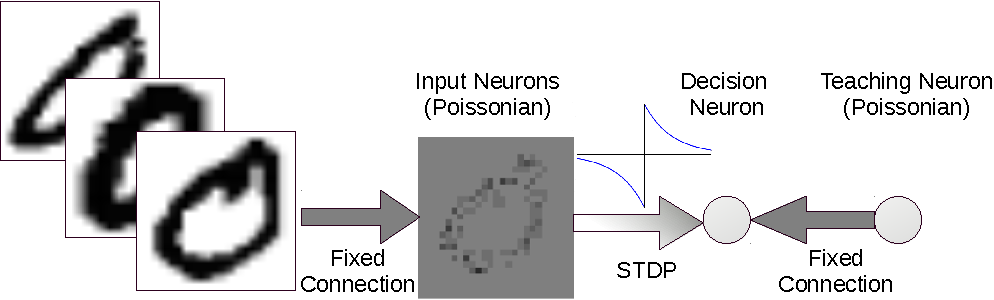
\includegraphics[width=0.48\textwidth]{training}
	} \\
	
	\centering
	
	\subfloat[Testing model of the spiking neural network.]{
		\label{Fig:test}
		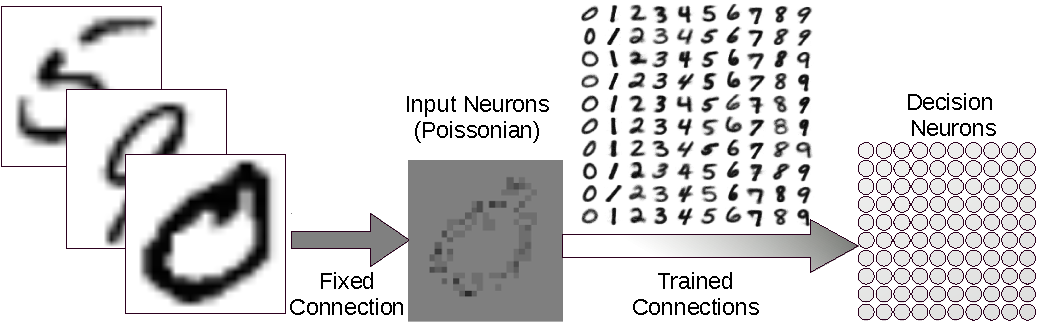
\includegraphics[width=0.48\textwidth]{testing}
	}
	
	\caption{The training and testing model of the two-layered spiking neural network.}
	\label{fig:model}
\end{figure} 



\subsubsection{Testing}
After training the weights of the plastic synapses are set to static, keeping the state of the weights at the last moment of training.
The weak weights were set to inhibitory connections with an identical strength.
The feed-forward testing network is shown in Fig.~\ref{Fig:test} where Poissonion spike trains are generated the same way as in the training with a total firing rate of $2,000$~Hz per image.
The input neurons convey the same spike trains to every decision neuron through its responding trained synaptic weights. 
Every testing image ($10,000$ images in total) is presented once and lasts 1~s with a silence of 200~ms between them.
The output neuron with the highest firing rate decides what digit was recognized.
Taken the trained weights from the NEST simulation, the accuracy of the recognition on NEST reaches 90.03\% with the standard configuration, while the result drops slightly to 89.97\% using SpiNNaker.
In comparison, both trained and tested on SpiNNaker the recognition accuracy is 87.41\%, and with the same weights applied to NEST the result turns out to be 87.25\%. 

\subsubsection{Evaluation}
The evaluation starts from the hardware-independent side, focusing on the spike-based recognition analysis.
As mentioned in Section~\ref{subsec:model}, CA and response time (latency) are the main concerns when assessing the recognition capability.
In our experiment, two sets of weights were applied: the original STDP trained weights and scaled-up weights which are 10 times stronger.
The spiking rates of the testing samples were also modified, ranging from 10 to $5,000$~Hz.

We found that accuracy depends largely on the time each sample is exposed to the network and the sample spiking rate (Fig.~\ref{fig:assess}.)
Furthermore, the latency of the output of the decision neurons is affected by both the spiking rate and connection weights.
Fig.~\ref{fig:acc_time} shows that the CA is better as exposure time increases. The longer an image is presented, the more information is gathered by the network, so the accuracy climbs.
Classification accuracy also increases when input spiking rates are augmented (Fig.~\ref{fig:acc_rate}.) Given that the spike trains injected into the network are more intense, the decision neurons become more active and so does the output disparity among them.
Nonetheless, it is important to know that these increments in CA have a limit, as is shown in the aforementioned figures.
With stronger weights, the accuracy is much higher when the input firing rate is less than $2,000$~Hz.


The latency of an SNN model is the result of the input rates and synaptic weights.
As the input rates grow, there are more spikes arriving at the decision neurons, triggering them to spike sooner.
A similar idea applies to the influence of synaptic weights. If stronger weights are taken, then the membrane potential of a neuron reaches its threshold earlier.
Fig.~\ref{fig:lat_rate} indicates that the latency is shortened with increasing input rates with both the original and scaled-up weights.
When the spiking rate is less than $2,000$~Hz, the network with stronger weights has a much shorter latency.
As long as there are enough spikes to trigger the decision neurons to spike, increasing the test time will not make the network respond sooner~(Fig.~\ref{fig:lat_time}.)
\begin{figure}[htb!]
	\centering
	\subfloat[Accuracy changes against test time.]{
		\label{fig:acc_time}
		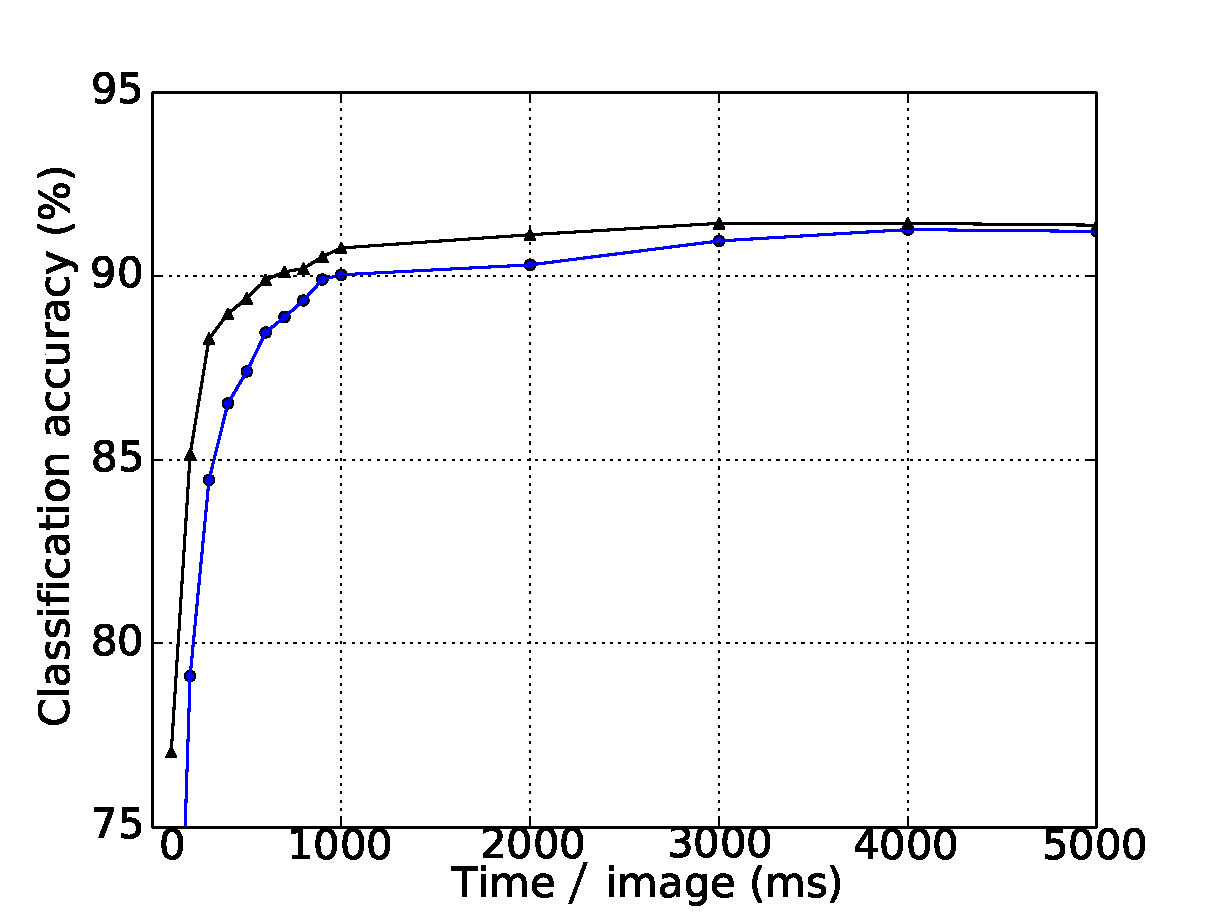
\includegraphics[width=0.25\textwidth]{acc_dur}
	}
	\subfloat[Accuracy changes against firing rate.]{
		\label{fig:acc_rate}
		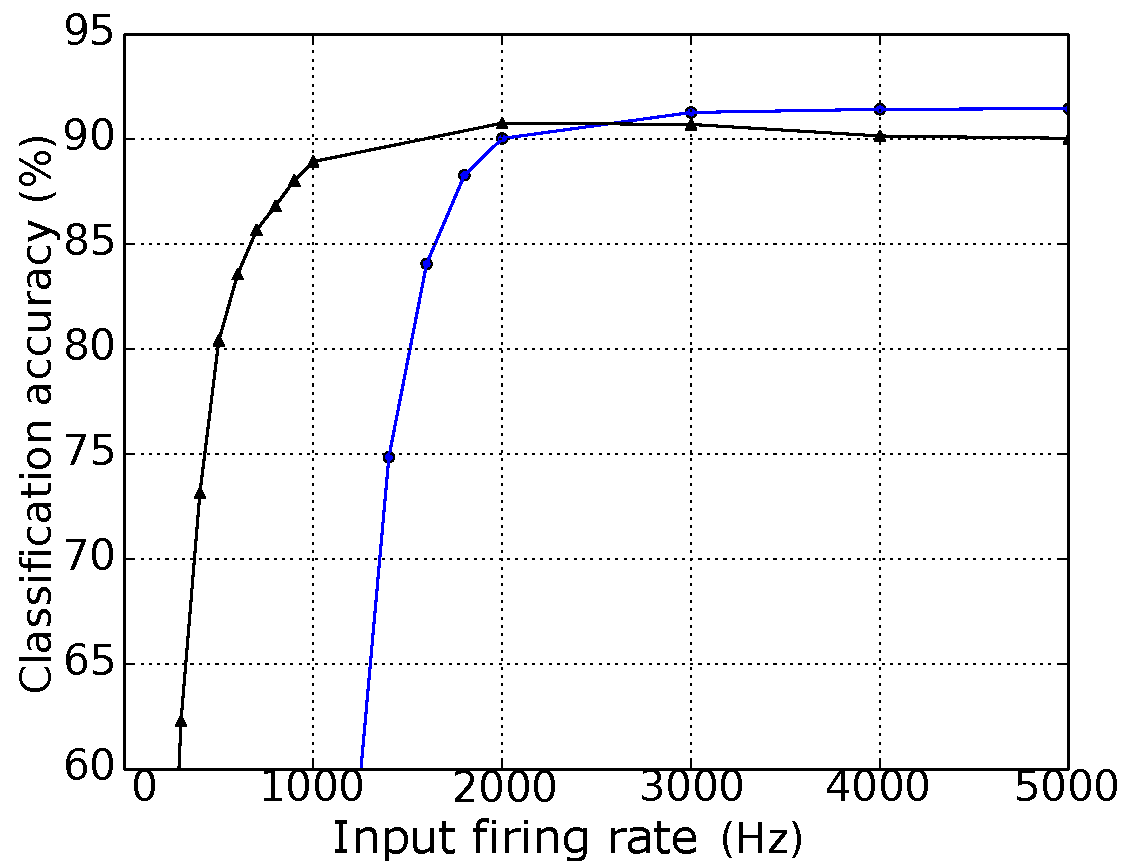
\includegraphics[width=0.25\textwidth]{acc_rate}
	}
	\\
	\subfloat[Latency stablises against test time.]{
		\label{fig:lat_time}
		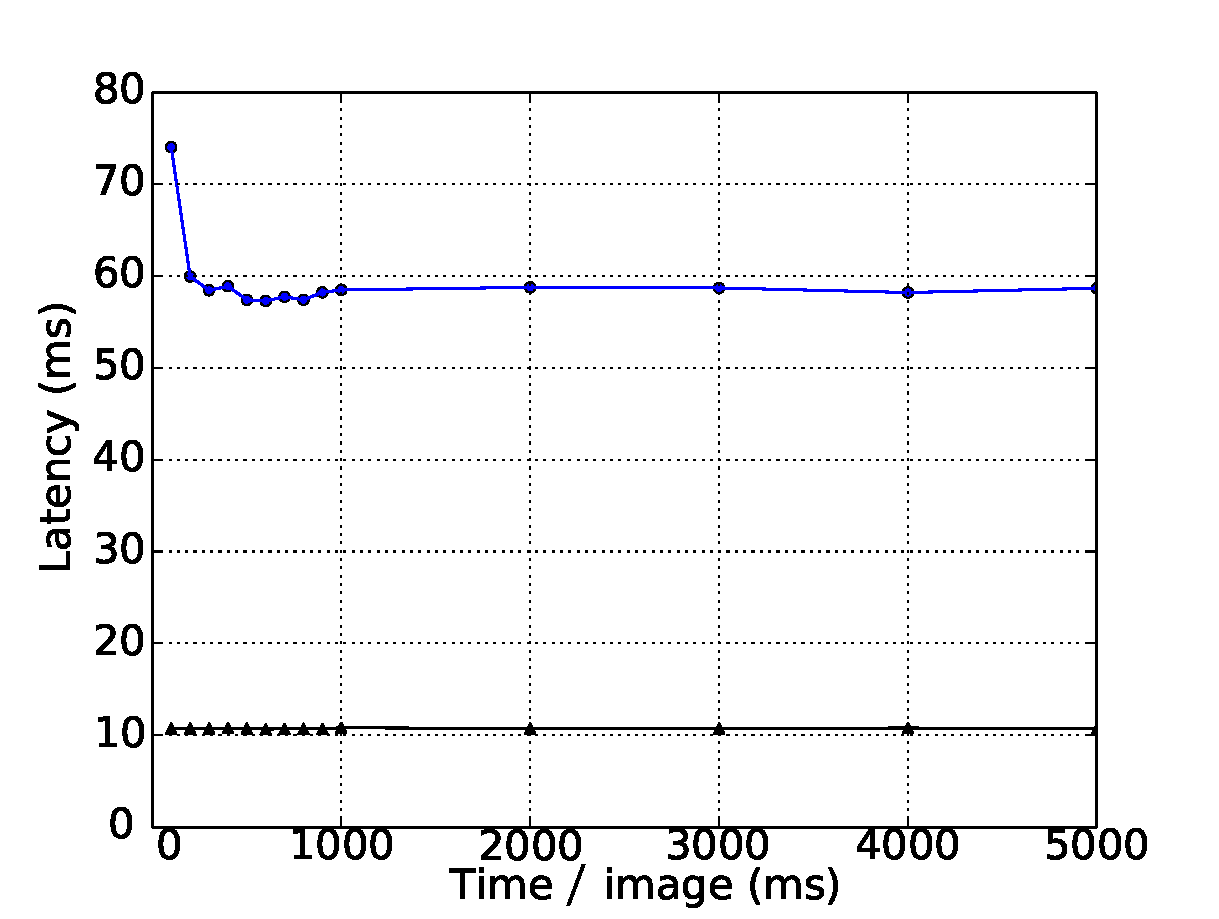
\includegraphics[width=0.25\textwidth]{lat_dur}
	}
	\subfloat[Latency changes against firing rate.]{
		\label{fig:lat_rate}
		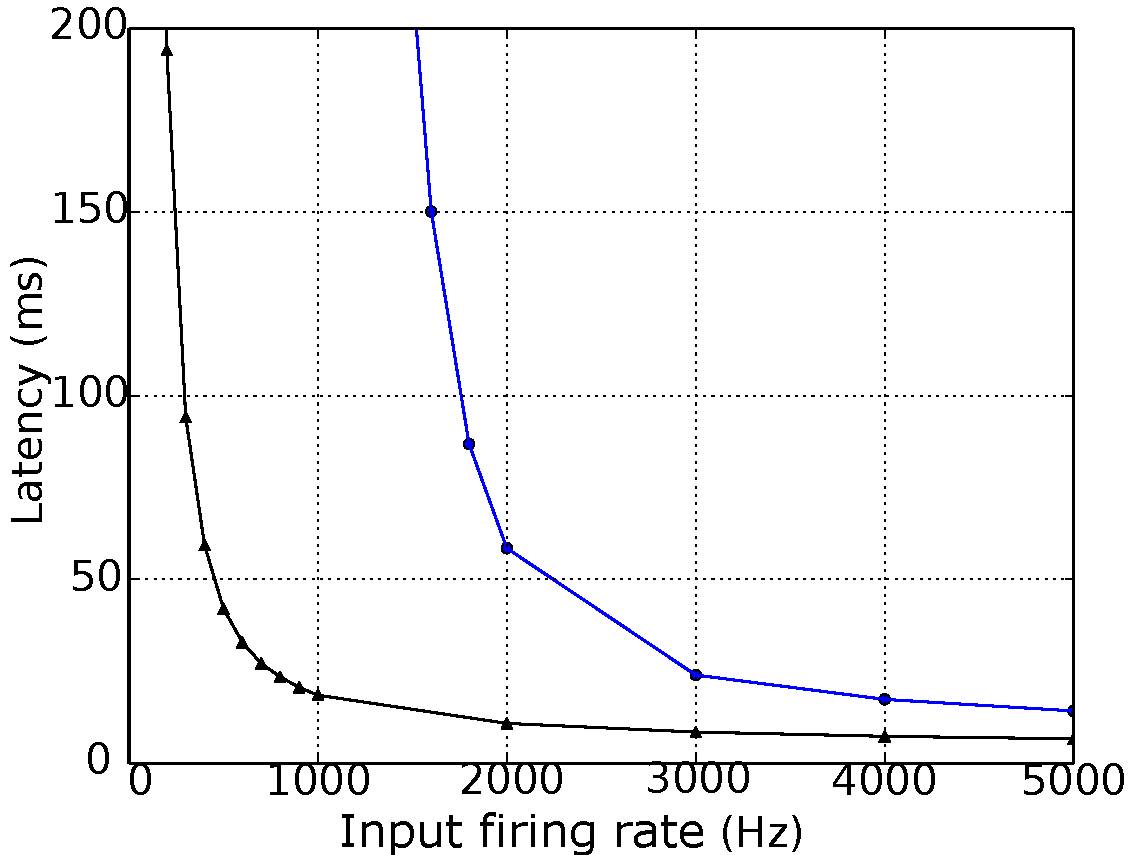
\includegraphics[width=0.25\textwidth]{lat_rate}
	}
	\caption{Accuracy and response time (latency) change over test time and input firing rate per testing image. Original trained weights are used (circles in blue) as well as the scaled up ($\times10$) weights (triangles in black). }
	\label{fig:assess}
\end{figure}

Regarding the network size, it not only influences the accuracy of a model but also the time taken for simulation on specific platforms thus impacting the energy usage on the hardware.
For the purpose of comparing the accuracy, simulation time and energy usage, different configurations have been tested on NEST (working on a PC with CPU: i5-4570 and 8G memory) and SpiNNaker, see Table~\ref{tbl:compare}.
The input rates in all of the tests are $5,000$~Hz, and each image is presented for 1~s.
The configurations only differ in the number of templates (subclasses/clusters) per digit.
The recognition accuracies differ in a range of $\pm0.5\%$ between NEST and SpiNNaker due to the limited fast memory and the necessity for fixed-point arithmetic on SpiNNaker to ensure real-time operation.
It is inevitable that numerical precision will be below IEEE double precision at various points in the processing chain from synaptic input to membrane potential.
The main bottleneck is currently in the ring buffer where the total precision for accumulated spike inputs is 16-bit, meaning that individual spikes are realistically going to be limited to 11- to 14-bit depending upon the probabilistic headroom calculated as necessary from the network configuration and spike throughput~\citep{Hopkins2015Accuracy}.
As the network size grows there are more decision neurons and synapses connecting to them, thus the simulation time on NEST increases.
On the other hand, SpiNNaker works in real (biologically real) time and the simulation time becomes shorter than NEST simulation when $1,000$ patterns per digit are used.
The Thermal Design Power (TDP) usage of all four processors of i5-4570 actively operating at base frequency is 84~W\footnote{\url{http://ark.intel.com/products/75043/Intel-Core-i5-4570-Processor-6M-Cache-up-to-3_60-GHz}}.
NEST was run fully active on a single core which cost 21~W of power usage.
The energy use can be calculated as the product of the simulation time and the power use.
Even with the smallest network, SpiNNaker wins in the energy cost comparison, see Fig.~\ref{fig:energy}.
Among different network configurations, the network of 500 decision neurons (50 clusters per digit) reaches the highest recognition rate.
%The recognition accuracy reaches the highest (92.98\%) when 50 patterns are trained per digit.
The network achieved a CA of 92.98\% and average latency of 10.70~ms, and the simulation costs SpiNNaker 0.41~W on power use and $4,920$~J on energy use.

\begin{table}[h]
	\caption{Comparisons of NEST (N) on a PC and SpiNNaker (S) performances.}
	\begin{center}
		\begin{tabular} {r|c|c|c|c|c|c}
			Subclasses
			&\multicolumn{2}{c|}{Accuracy (\%)}  &\multicolumn{2}{c|}{Simulation (s)}
			&\multicolumn{2}{c}{Power Use (W)}   \\
			\cline{2-7}
			per digit
			& N & S & N & S & N & S\\
			\hline
			1 & 79.62 & 79.50 & 554.77 & \multirow{5}{*}{$12,000$} & \multirow{5}{*}{ 21.0 } & 0.38 \\
			10 & 91.29 & 91.43 & 621.74 &   &   & 0.38 \\
			50 & 92.98 & 92.92 & $1,125.12$ &   &   & 0.41 \\
			100 & 87.27 & 86.83 & $1,406.01$ &   &   & 0.44 \\
			1000 & 89.65 & 89.74 & $30,316.88$ &   &   & 1.50 \\
			
		\end{tabular}
		\label{tbl:compare}
	\end{center}
\end{table}

\begin{figure}[hbt!]
	\centering
	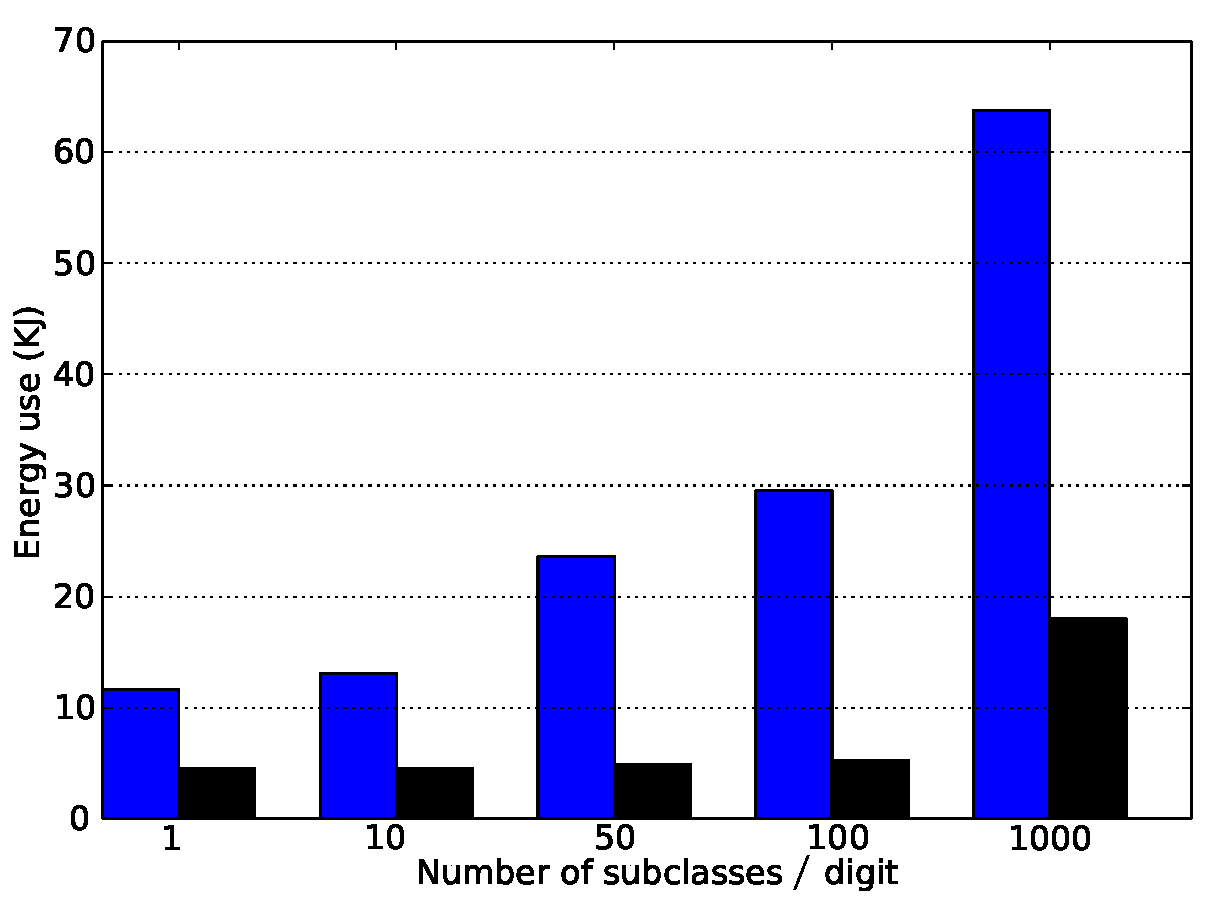
\includegraphics[width=0.48\textwidth]{energy}
	\caption{Energy usages of different network size both using NEST (blue) on a PC and SpiNNaker (black).}
	\label{fig:energy}
\end{figure}
\subsection{Case Study II}
% brief intro about dbn
Deep learning architectures and in particular Convolutional Networks~\citep{lecun1998gradient} and Deep Belief Networks (DBNs)~\citep{hinton2006fast} have been characterised as one of the breakthrough technologies of the decade~\citep{MIT_TechReview}. One of the advantages of these type of networks is that their performance can be increased by adding more layers~\citep{hinton2006fast}.

However, state-of-the-art deep networks comprise a large number of layers, neurons and connections resulting in high energy demands, communication overheads, and high response latencies. This is a problem for mobile and robotic platforms which may have limited computational and power resources but require fast system responses. 


% about oneils model 
\citet{o2013real} proposed a method to map off-line trained DBNs into a spiking neural networks and take advantage of the real-time performance and energy efficiency of neuromorphic platforms. This led initially to an implementation on an event-driven Field-Programmable Gate Array (FPGA) called Minitaur~\citep{neil2014minitaur} and then on the SpiNNaker platform~\citep{Stromatias2015scalable}. For this work we used an off-line trained\footnote{\url{https://github.com/dannyneil/edbn/}} spiking DBN with a 784-500-500-10 network topology. Simulations take place on a software spiking neural network simulator named Brian~\citep{goodman2008brian} and results are verified on the SpiNNaker platform.

\subsubsection{Training}

DBNs consist of stacked Restricted Boltzmann Machines (RBMs), which are fully connected recurrent networks but without any connections between neurons of the same layer. Training is performed unsupervised using the standard CD rule~\citep{hinton2006fast} and only the output layer is trained in a supervised manner. The main difference between spiking DBNs and traditional DBNs is the activation function used for the neurons.~\cite{o2013real} proposed the use of the Siegert approximation~\citep{Jug_etal_2012} as the activation function, which returns the expected firing rate of a LIF neuron given input firing rates, input weights, and standard neuron parameters.

\subsubsection{Testing}
After the training process the learnt synaptic weights can be used in a spiking neural network which consists of LIF neurons with delta-current synapses. Table~\ref{Tab:NeuralParams} shows the LIF parameters used in the simulations.

\begin{table}[hbbp]
	\centering
	\caption{\label{Tab:NeuralParams}Default parameters of the Leaky Integrate-and-Fire Model used in simulations.}
	\bgroup
	\def\arraystretch{1.1}
	\begin{tabular}{c|c|c}
		%\hline
		Parameters & Values & Units \\
		\hline
		tau\_m & 5 & s\\
		%\hline
		tau\_refrac & 2.0 & ms\\
		%\hline
		v\_reset & 0.0 & mV\\
		%\hline
		v\_rest & 0.0 & mV\\
		%\hline
		v\_thresh & 1.0 & mV\\
		%\hline
	\end{tabular}
	\egroup
\end{table}

The pixels of each MNIST digit from the testing set are converted into Poisson spike trains with a rate proportional to the intensity of their pixel, while their firing rates are scaled so that the total firing rate of the input population is constant~\citep{o2013real}.

The CA was chosen as the performance metric of the spiking DBN, which is the percentage of the correctly classified digits over the whole MNIST testing set.

\subsubsection{Evaluation}
Neuromorphic platforms may have limited hardware resources to store the synaptic weights~\citep{schemmel2010wafer,merolla2014million}. In order to investigate how the precision of the weights affects the CA of a spiking DBN the double floating point weights of the offline trained network were converted to different fixed-point representations. The following notation will be used throughout this paper, Q\textit{m.f}, where \textit{m} signifies the number of bits for the integer part (including the sign bit) and \textit{f} the number of bits used for the fractional part.

Figure~\ref{Fig:brianCAfiringrate} shows the effect of reduced weight bit precision on the CA for different input firing rates on the Brian simulator.
%To validate the results of the software simulator simulations ran on SpiNNaker for a weight resolution of Q3.8.
Using the same weight precision of Q3.8, SpiNNaker achieved a CA of 94.94\% when $1,500$~Hz was used for the input population~\citep{Stromatias2015scalable}. Brian for the same firing rates and weight precision achieved a CA of 94.955\%. Results are summarised in Table~\ref{tab:casimulators}.
The slightly lower CA of the SpiNNaker simulation indicates that not only the weight precision but also the precision of the membrane potential affects the overall classification performance.    

\begin{figure}[hbt!]
	\centering
	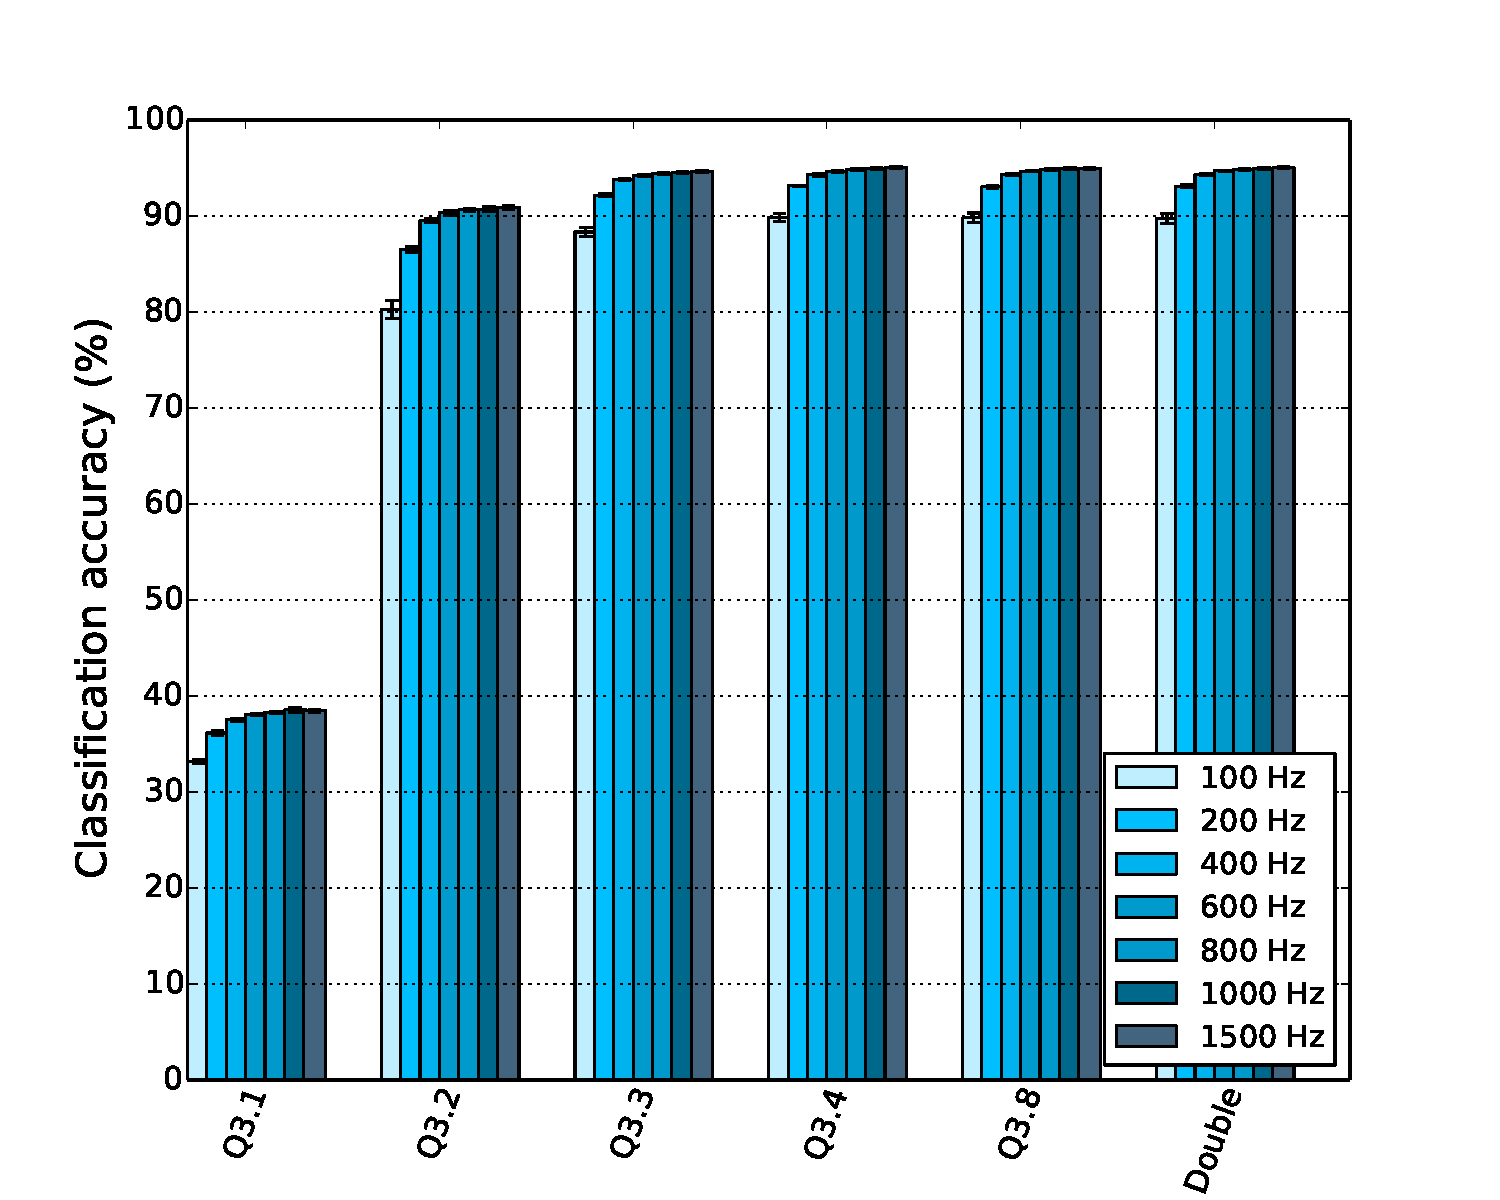
\includegraphics[width=0.48\textwidth]{cavsfiringrate}
	\caption{CA as a function of the weight bit precision for different input firing rates.}
	\label{Fig:brianCAfiringrate}
\end{figure} 


\begin{table}[h]
	\caption{Classification accuracy (CA) of the same DBN running on different platforms.}
	\begin{center}
		\begin{tabular} {c|c|c}
			Simulator & CA (\%) & Weight Precision \\
			\hline
			Matlab & 96.06 & Double floating point\\
			Brian & 95.00 & Double floating point\\
			Brian & 94.955 & Q3.8\\
			SpiNNaker & 94.94 & Q3.8\\
			%    \hline
		\end{tabular}
		\label{tab:casimulators}
	\end{center}
\end{table}

\citet{stromatias2015robustness} showed that spiking DBNs are capable of maintaining a high CA even for weight precisions down to Q3.3, while they are also remarkably robust to high levels of input noise regardless of the weight precision. 

A similar experiment to the one presented for the Case Study I was performed; its purpose was to establish the relation that input spike rates hold with latency and classification accuracy.
The input rates were varied from 500~Hz to $2,000$~Hz and the results are summarised in Figure~\ref{Fig:brianLatency}. Simulations ran in Brian for all $10,000$ MNIST digits of the testing set and for 4 trials. Figure~\ref{Fig:spinnLatency1500hz} shows a histogram of the classification latencies on SpiNNaker when the input rates are $1,500$~Hz. The mean classification latency for the particular spiking DBN on SpiNNaker is 16~ms which is identical to the Brian simulation seen in Figure~\ref{Fig:brianLatency}.


\begin{figure}[hbt!]
	\centering
	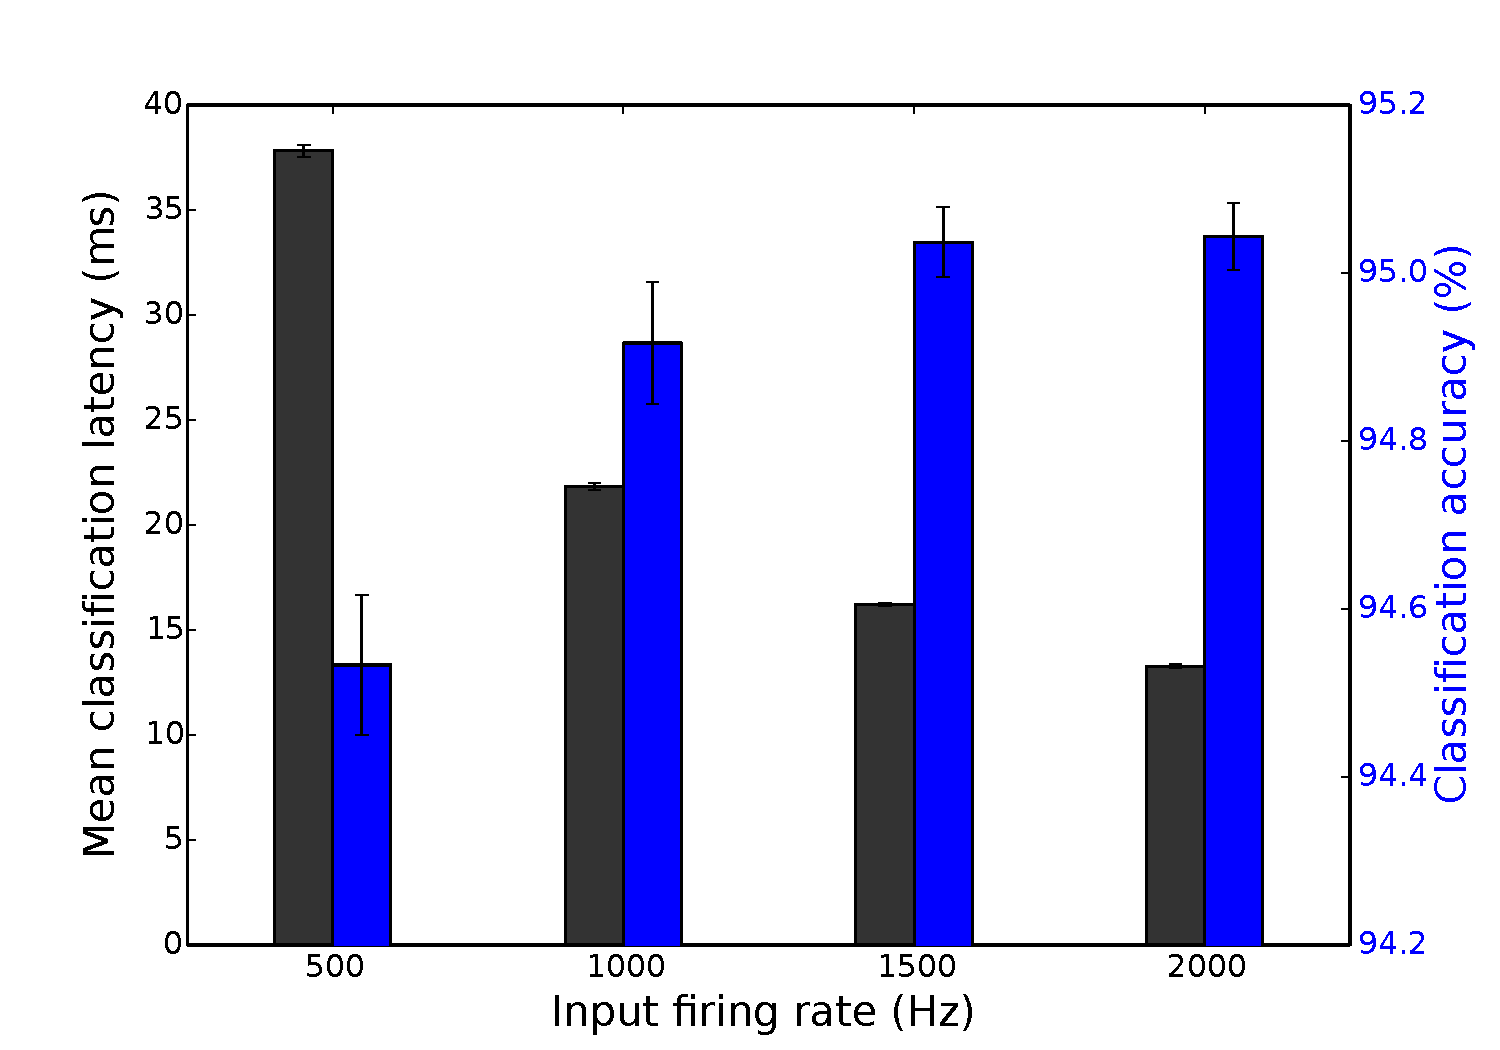
\includegraphics[width=0.48\textwidth]{latencyCAfiringrate}
	\caption{Mean classification latency (black) and classification accuracy (blue) as a function of the input firing rate for the spiking DBN. Results are averaged over 4 trials, error bars show standard deviations.}
	\label{Fig:brianLatency}
\end{figure} 



\begin{figure}[hbt!]
	\centering
	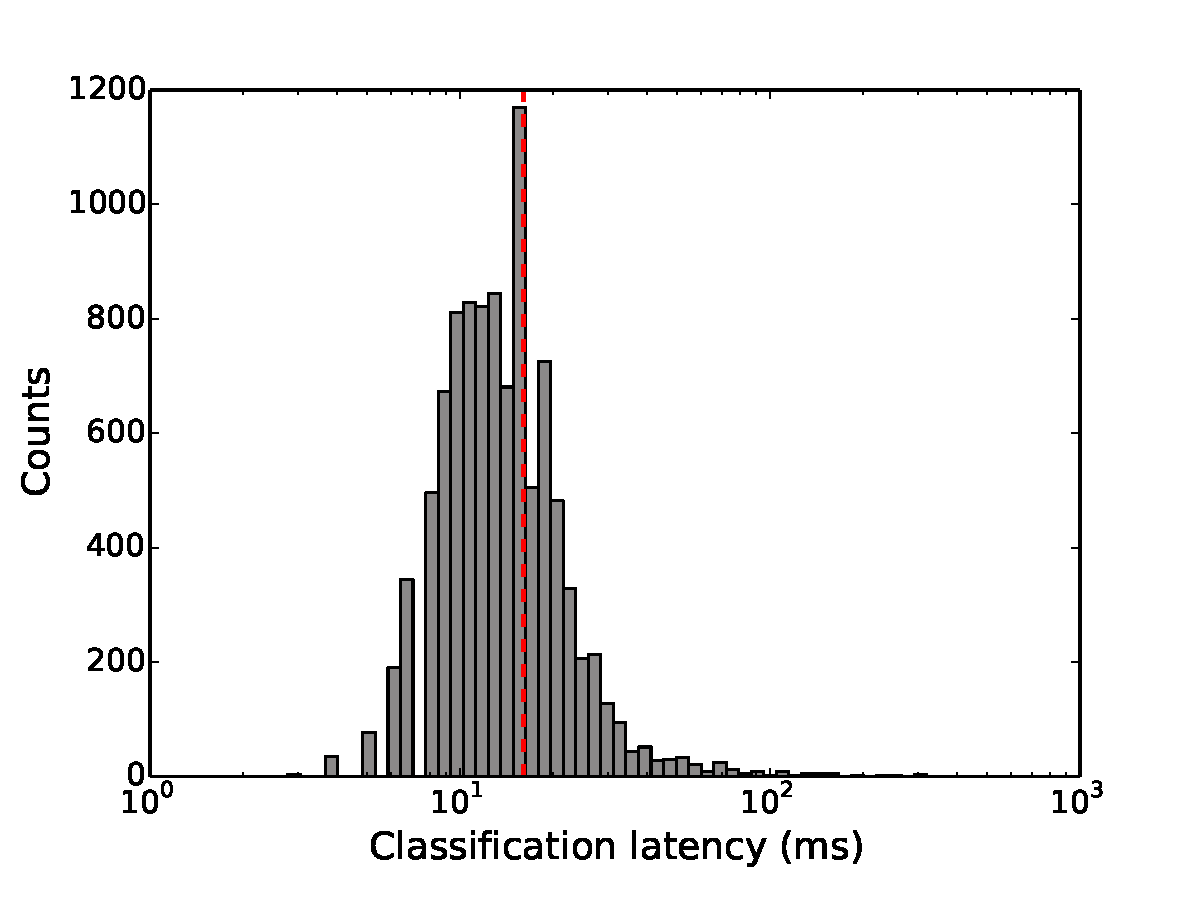
\includegraphics[width=0.48\textwidth]{classlatencyIJCNN1500hz}
	\caption{Histogram of the classification latencies for the MNIST digits of the testing set when the input rates are set to $1,500$~Hz. The mean classification latency of the spiking DBN on SpiNNaker is 16 ms.}
	\label{Fig:spinnLatency1500hz}
\end{figure} 

Finally, this particular spiking DBN ran on a single SpiNNaker chip (16 ARM9 cores) and dissipated less than 0.3~W when $2,000$ spikes per second per digit were used, as seen in Figure~\ref{Fig:spinnchipPower}. The identical network ran on Minitaur~\citep{neil2014minitaur}, an event-driven FPGA implementation, and consumed 1.5~W when $1,000$ spikes per image were used.  


\begin{figure}[hbt!]
	\centering
	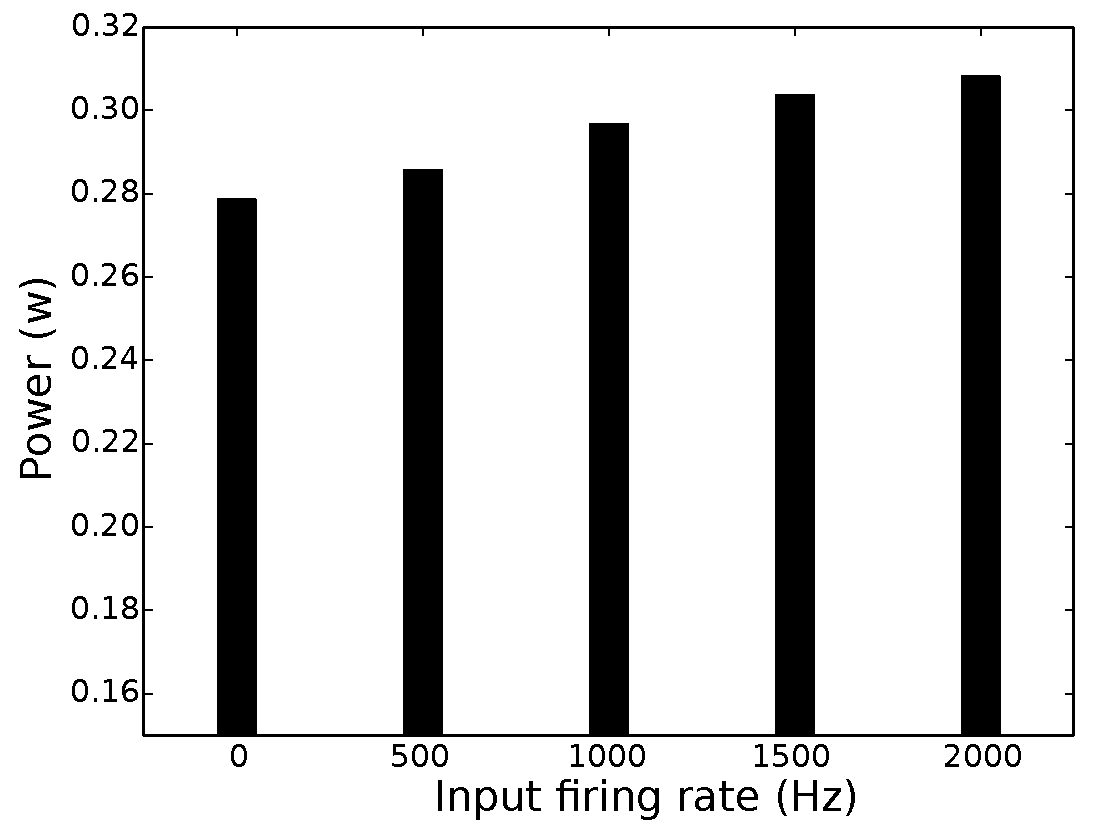
\includegraphics[width=0.48\textwidth]{powerspinnaker}
	\caption{Power dissipation of a spiking DBN running on a single SpiNNaker chip as a function of the total input firing rate.}
	\label{Fig:spinnchipPower}
\end{figure} 

\section{Conclusion}
\label{sec:summ}
\subsection{What we have said and done}
This paper puts forward the NE dataset as a baseline for comparisons on vision based SNNs.
It contains converted spike representations of existing widely-used databases in the vision recognition field.
Since new problems will be introduced continuously before vision becomes a solved question, the dataset will evolve as research develops. 
The conversion methods transforming images and videos to spike trains will advance. The number of vision databases included will increase and the corresponding evaluation methodology will evolve as well.
The dataset aims to provide a unified spike-based vision database and complementary evaluation methodologies to assess the performance of various SNN algorithms.

The first launch of the dataset is published as NE15-MNIST, which contains four different spike presentations of the stationary hand-written digit database.
The Poissonian subset aims at benchmarking the existing rate-based recognition methods.
The rank-order-encoded subset, FoCal, encourages research into spatio-temporal algorithms on recognition applications using only small numbers of input spikes.
Fast recognition can be verified on the subset of DVS recorded flashing input, since merely 30~ms of useful spike trains are recorded for each image.
As a step forward, the continuous spike trains captured from the DVS recorded moving input can be a good test on mobile neuromorphic robots.

The complementary evaluation methodology is essential to assess both the model-level and hardware-level performances.
For a network model, its topology, neuron and synapse models, and training methods are major descriptions for any kind of neural networks, including SNNs.
While the recognition accuracy, network latency and also the biological time taken for both training and testing are specific performance measurements of a spike-based model.
To build any SNN model on a hardware platform, its network size will be constrained by the scalability of the hardware. Neural and synaptic models are limited to the ones that are physically implemented, unless the hardware platform supports programmability.
The accuracy of the results (e.g. CA) are naturally affected by the precision of the variable representing the membrane potential and synaptic weights.
Any attempt to implement an on-line learning algorithm on neuromorphic hardware must be backed by synaptic plasticity support.
Running an identical SNN model on different neuromorphic hardware platforms can not only expose if any of the previously mentioned capacities are supported, but also benchmark their performance on simulation time and energy usage.

Using the Poissonian subset of the NE15-MNIST dataset, two benchmark systems were proposed. 
The models were described and their performance on accuracy, network latency, simulation time and energy usage were presented.
These example benchmarking systems provided a recommended way of using the dataset and evaluating system performance.
They provide a baseline for comparisons and encourage improved algorithms and models to make use of the dataset.

Although spike-based algorithms have not surpassed their non-spiking counterparts in terms of recognition accuracy, they have shown great performance in response time and energy efficiency.
The dataset makes the comparison of SNNs with conventional recognition methods possible by using converted spike presentations of the same vision databases.
As the dataset grows, it will allow new problems to be investigated by researchers, which should allow the identification of future directions and, in consequence, advance the field.

%\subsection{The future direction of a developing database}
\subsection{The future direction of an evolving database}
The database will expand by converting more popular vision datasets to spike representations.
As mentioned in Section~\ref{sec:intro}, face recognition has become a hot topic in SNN approaches, however there is no unified spike-based dataset to benchmark theses networks.
Thus, the next development step for our dataset is to include face recognition databases.
While viewing an image,  saccades direct high-acuity visual analysis to a particular object or a region of interest and useful information is gathered during the fixation of several saccades in a second.
It is possible to measure the scan path or trajectory of the eyeball and the trajectories showed particular interest in eyes, nose and mouth while viewing a human face~\citep{yarbus1967eye}.
Therefore, our plan is also to embed modulated trajectory information to direct the recording using DVS sensors to simulate human saccades.


%While the major stumbling crux of the computer object recognition systems lies in the invariance problem.
Each encounter of an object on the retina is completely unique, because of the illumination (lighting conditions), position (projection locations on the retina), scale (distances and sizes), pose (viewing angles), and clutter (visual contexts) variabilities.
But the brain recognises a huge number of objects rapidly and effortlessly even in cluttered and natural scenes.
In order to explore invariant object recognition, the dataset is going to include the NORB (NYU Object Recognition Benchmark) dataset~\citep{lecun2004learning}, which contains images of objects that are first photographed in ideal conditions and then moved and placed in front of natural scene images.

Action recognition will be the first problem of video processing to be introduced in the dataset.
The initial plan is to use the DVS retina to convert KTH and Weizmann benchmarks to spiking versions.
Meanwhile, providing a software DVS retina simulator to transform  frames into spike trains is also on the schedule.
By doing this, huge number of videos, such as in YouTube, can automatically be converted to spikes, therefore providing researchers more time to work on their own applications.



\section*{Acknowledgments}

The work presented in this paper was largely inspired by discussions at the 2015 Workshops on Neuromorphic Cognition Engineering in CapoCaccia.
The authors would like to thank the organisers and the sponsors.
The authors would also like to thank Patrick Camilleri, Michael Hopkins, and John Woods for the meaningful discussions and proofreading of the paper.
The construction of the SpiNNaker machine was supported by the Engineering and Physical Science Research Council (EPSRC grant EP/4015740/1) with additional support from industry partners ARM Ltd and Silistix Ltd.
The research leading to these results has received funding from the European Research Council under the European Union's Seventh Framework Programme (FP/2007-2013) / ERC Grant Agreement n. 320689 and also from the EU Flagship Human Brain Project (FP7-604102). 

\bibliographystyle{frontiersinSCNS&ENG} % for Science and Engineering articles
%\bibliographystyle{frontiersinMED} % for Medicine articles

\bibliography{bench_ref}
%\bibliography{ref,rank-ordered,hw-ind-eval,hw-dep-eval,bench_ref}

\end{document}
